% Options for packages loaded elsewhere
\PassOptionsToPackage{unicode}{hyperref}
\PassOptionsToPackage{hyphens}{url}
%
\documentclass[
]{article}
\usepackage{amsmath,amssymb}
\usepackage{lmodern}
\usepackage{iftex}
\ifPDFTeX
  \usepackage[T1]{fontenc}
  \usepackage[utf8]{inputenc}
  \usepackage{textcomp} % provide euro and other symbols
\else % if luatex or xetex
  \usepackage{unicode-math}
  \defaultfontfeatures{Scale=MatchLowercase}
  \defaultfontfeatures[\rmfamily]{Ligatures=TeX,Scale=1}
\fi
% Use upquote if available, for straight quotes in verbatim environments
\IfFileExists{upquote.sty}{\usepackage{upquote}}{}
\IfFileExists{microtype.sty}{% use microtype if available
  \usepackage[]{microtype}
  \UseMicrotypeSet[protrusion]{basicmath} % disable protrusion for tt fonts
}{}
\makeatletter
\@ifundefined{KOMAClassName}{% if non-KOMA class
  \IfFileExists{parskip.sty}{%
    \usepackage{parskip}
  }{% else
    \setlength{\parindent}{0pt}
    \setlength{\parskip}{6pt plus 2pt minus 1pt}}
}{% if KOMA class
  \KOMAoptions{parskip=half}}
\makeatother
\usepackage{xcolor}
\usepackage[margin=1in]{geometry}
\usepackage{graphicx}
\makeatletter
\def\maxwidth{\ifdim\Gin@nat@width>\linewidth\linewidth\else\Gin@nat@width\fi}
\def\maxheight{\ifdim\Gin@nat@height>\textheight\textheight\else\Gin@nat@height\fi}
\makeatother
% Scale images if necessary, so that they will not overflow the page
% margins by default, and it is still possible to overwrite the defaults
% using explicit options in \includegraphics[width, height, ...]{}
\setkeys{Gin}{width=\maxwidth,height=\maxheight,keepaspectratio}
% Set default figure placement to htbp
\makeatletter
\def\fps@figure{htbp}
\makeatother
\setlength{\emergencystretch}{3em} % prevent overfull lines
\providecommand{\tightlist}{%
  \setlength{\itemsep}{0pt}\setlength{\parskip}{0pt}}
\setcounter{secnumdepth}{-\maxdimen} % remove section numbering
\newlength{\cslhangindent}
\setlength{\cslhangindent}{1.5em}
\newlength{\csllabelwidth}
\setlength{\csllabelwidth}{3em}
\newlength{\cslentryspacingunit} % times entry-spacing
\setlength{\cslentryspacingunit}{\parskip}
\newenvironment{CSLReferences}[2] % #1 hanging-ident, #2 entry spacing
 {% don't indent paragraphs
  \setlength{\parindent}{0pt}
  % turn on hanging indent if param 1 is 1
  \ifodd #1
  \let\oldpar\par
  \def\par{\hangindent=\cslhangindent\oldpar}
  \fi
  % set entry spacing
  \setlength{\parskip}{#2\cslentryspacingunit}
 }%
 {}
\usepackage{calc}
\newcommand{\CSLBlock}[1]{#1\hfill\break}
\newcommand{\CSLLeftMargin}[1]{\parbox[t]{\csllabelwidth}{#1}}
\newcommand{\CSLRightInline}[1]{\parbox[t]{\linewidth - \csllabelwidth}{#1}\break}
\newcommand{\CSLIndent}[1]{\hspace{\cslhangindent}#1}
\usepackage{lineno}
\linenumbers
\usepackage{setspace}\doublespacing
\usepackage{gensymb}
\usepackage{caption}
\captionsetup[figure]{labelformat=empty}
\usepackage[nomarkers, nolists, figuresonly]{endfloat}
\usepackage{float}
\ifLuaTeX
  \usepackage{selnolig}  % disable illegal ligatures
\fi
\IfFileExists{bookmark.sty}{\usepackage{bookmark}}{\usepackage{hyperref}}
\IfFileExists{xurl.sty}{\usepackage{xurl}}{} % add URL line breaks if available
\urlstyle{same} % disable monospaced font for URLs
\hypersetup{
  pdftitle={Quantifying Impacts of an Environmental Intervention Using Environmental DNA: Supplemental Text 1},
  pdfauthor={Elizabeth Andruszkiewicz Allan,; Ryan P. Kelly,; Erin D'Agnese,; Maya Garber-Yonts,; Megan Shaffer,; Zachary Gold,; Andrew O. Shelton},
  hidelinks,
  pdfcreator={LaTeX via pandoc}}

\title{Quantifying Impacts of an Environmental Intervention Using
Environmental DNA: Supplemental Text 1}
\author{Elizabeth Andruszkiewicz Allan, \and Ryan P. Kelly, \and Erin
D'Agnese, \and Maya Garber-Yonts, \and Megan Shaffer, \and Zachary
Gold, \and Andrew O. Shelton}
\date{2023}

\begin{document}
\maketitle

\hypertarget{field-sampling}{%
\subsection{Field Sampling}\label{field-sampling}}

\hypertarget{site-selection-and-study-design}{%
\subsubsection{Site selection and study
design}\label{site-selection-and-study-design}}

There were two culverts in the treatment creek (Padden) that were
suspected to be partially impassible and thus was removed and replaced
during the course of the study; one of the control creeks had a bridge,
which allowed fish passage (Portage), one control creek had a culvert
classified as having limited fish passability (Squalicum), and two
control creeks had culverts classified as preventing fish passage
(Barnes and Chuckanut) (Washington Department of Fish and Wildlife
2019). These creeks were chosen due to their comparable size, flow,
watersheds, and species presumed to be present to constrain as many
ecological variables as possible.

\hypertarget{distance-between-sites-and-flow-variability-at-sites}{%
\subsubsection{Distance between sites and flow variability at
sites}\label{distance-between-sites-and-flow-variability-at-sites}}

The average distance between upstream and downstream sampling within a
creek was about 160 m; the largest distance between downstream and
upstream sampling was at Barnes Creek, which was approximately 330 m,
whereas the shortest distance between sampling was at Squalicum Creek at
approximately 66 m.

Over the course of the year, flow within each creek varied. USGS flow
gauges were located in three of the five creeks, relatively nearby to
the sampling locations (Figure S1.\ref{fig:gaugemap}). The closest gauge
to sampling locations was Padden Creek (\textasciitilde1.5 km); the
gauge at Chuckanut Creek was \textasciitilde5.5 km and the gauge at
Squalicum Creek was \textasciitilde7.9 km away (calculated using the
Haversine distance in R).

\begin{figure}
\centering
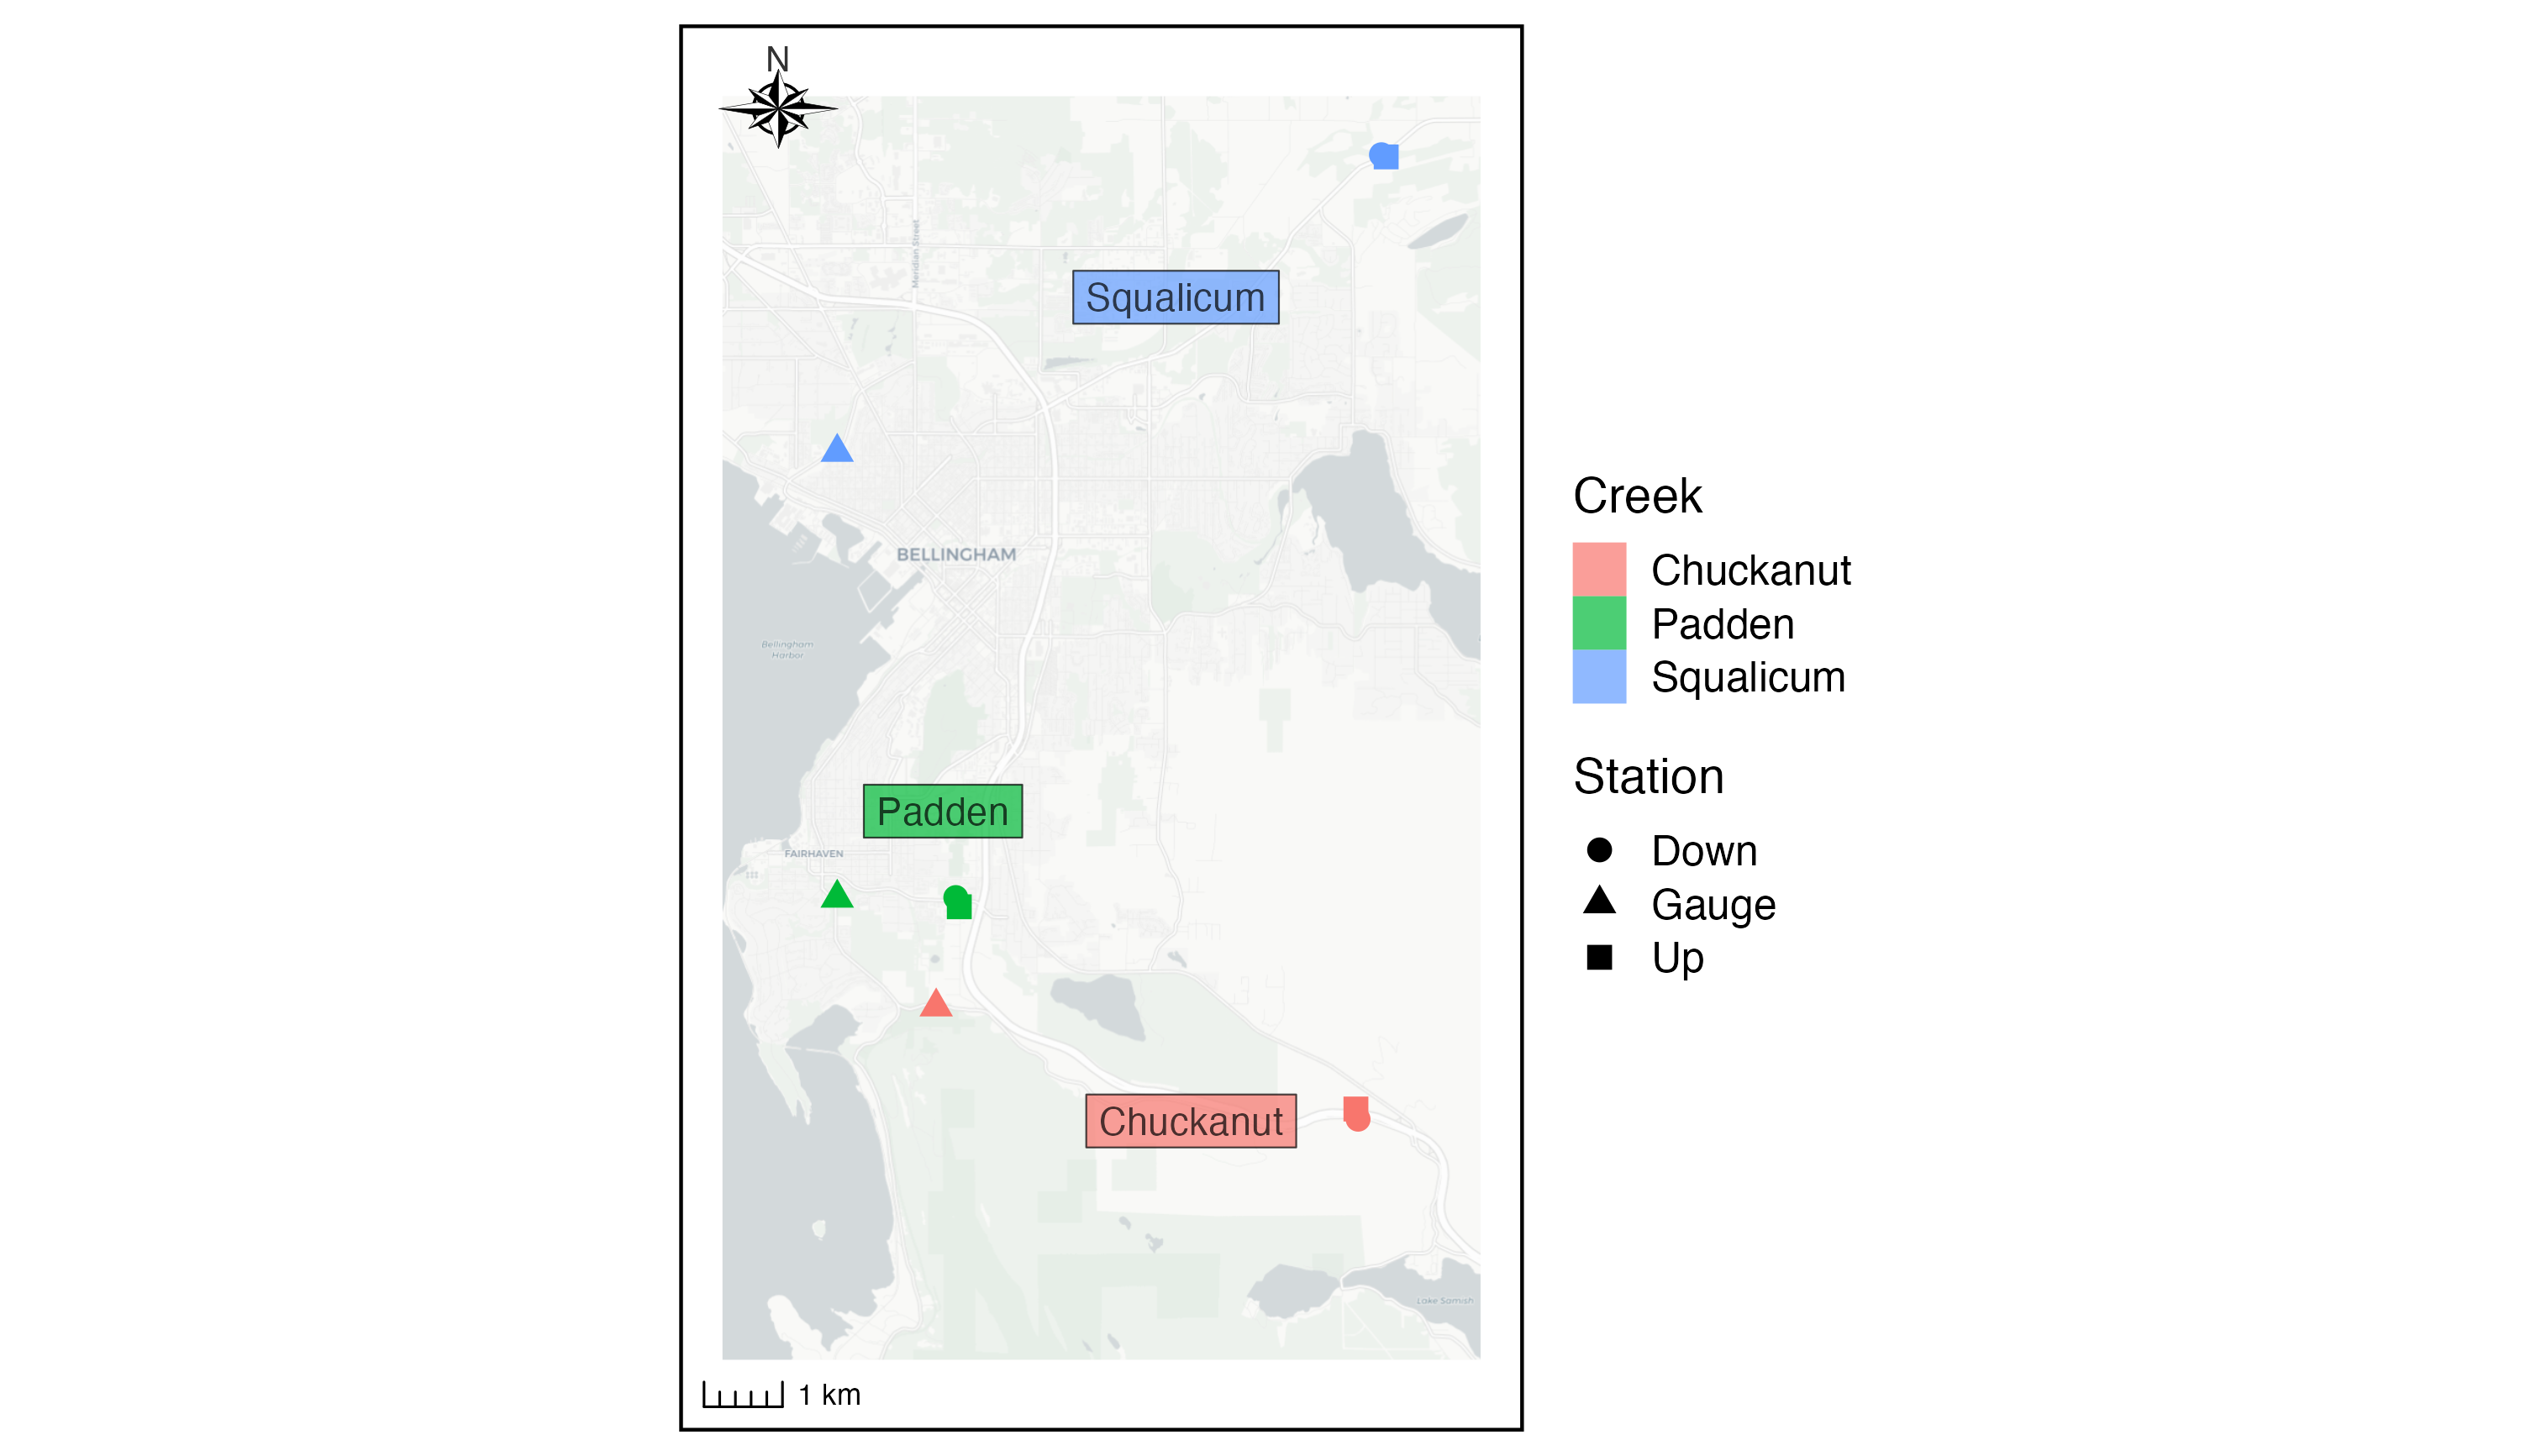
\includegraphics{../Output/SupplementalFigures/map_gauges.png}
\caption{Figure S1.1. Location of flow gauges compared to sampling
locations for Chuckanut, Padden, and Squalicum
Creeks.\label{fig:gaugemap}}
\end{figure}

The flow meters at Squalicum Creek and Chuckanut Creek were offline from
November 2021 for the remainder of the sampling period. The highest
discharge seen during the course of the study from January to November
2021 occurred in November 2021 at Squalicum Creek. The mean discharge in
each creek was: 0.42 m\textsuperscript{3}/s in Padden, 0.29
m\textsuperscript{3}/s in Chuckanut, and 1.14 m\textsuperscript{3}/s in
Squalicum Creek. The lowest discharge registered by the flow meters is
0.0028 m\textsuperscript{3}/s, which occurred 8.5\%, 1.6\%, and 0.78\%
of the time in Padden, Chuckanut, and Squalicum, respectively.

Due to the lack of flow data in Squalicum and Chuckanut Creeks from
November 2021 to February 2022, we used historical data from the three
flow gauges to calculate the average discharge for each day of the year
from about 2015-2021 (Figure S1.\ref{fig:dischargesupp}). We then used
the value for the day of the year that we sampled in either 2021 or 2022
when the gauges were offline. For consistency, we also did this at
Padden Creek despite the gauge there being online for the entire
sampling period.

\begin{figure}
\centering
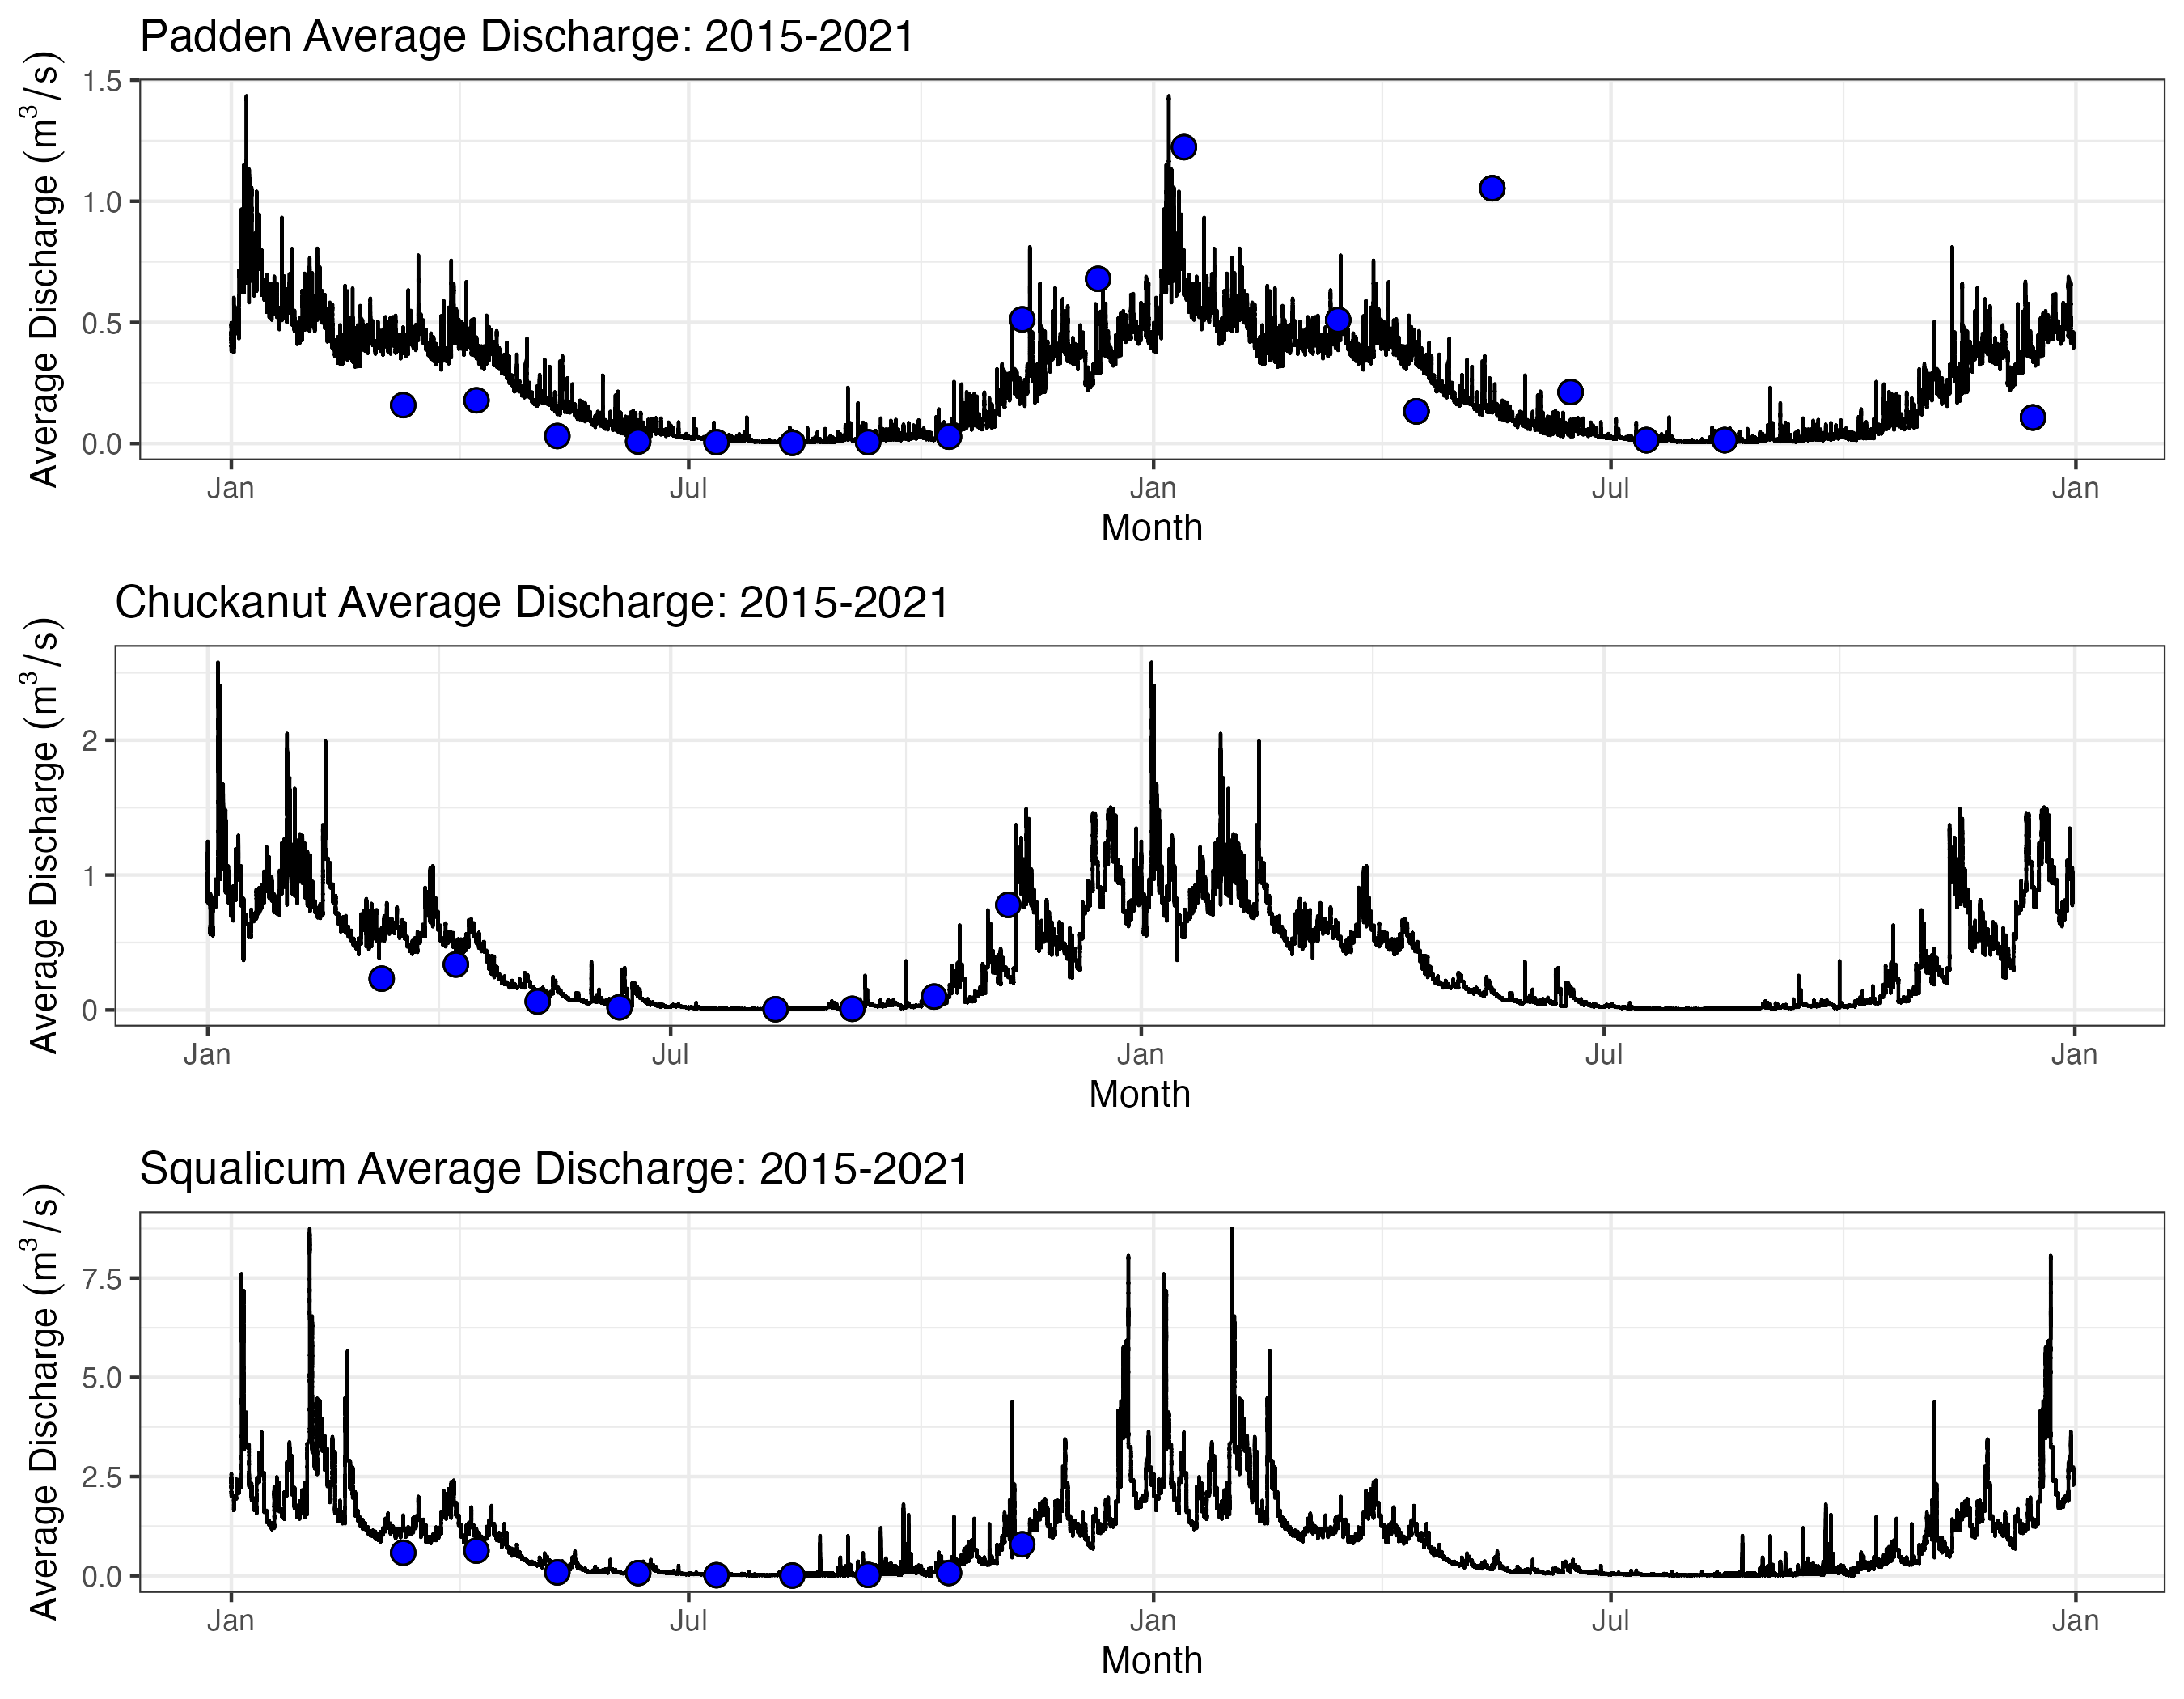
\includegraphics{../Output/SupplementalFigures/historical_flow_year_avg_sampling.png}
\caption{Figure S1.2. Daily average discharge from 2015-2020 in creeks
from USGS gauges. Blue dots show the discharge time of sampling during
the course of this study (2021-2022) for time points where gauges were
online (note the missing data points after December through February in
Chuckanut and Squalicum Creeks).\label{fig:dischargesupp}}
\end{figure}

We compared the different ways one could use flow data to correct the
eDNA concentrations. We included (1) the value from the closest time
point from the gauge to the time point sampling, (2) the average flow on
the day of sampling from the gauge, (3) the monthly average for the
month of sampling from the gauge, and (4) the correction factor
approach. For (4), the values for Padden Creek represent the same as (1)
for Padden Creek, the value from the closest time point in the gauge to
the time point of sampling. The values for Chuckanut and Squalicum Creek
are based on the the correction factor from Padden Creek. First, five
years of historical data (2015-2020) were used to find monthly averages
for flow rates for each creek. Because the gauges in Squalicum and
Chuckanut Creeks stopped metering in 2021, we solved for the ratio of
the monthly average of each of those creeks to Padden Creek. Then, we
used the closest values from Padden Creek (1) and multiplied by the
monthly correction factor from the 5 years of historical data to find a
value for Squalicum and Chuckanut Creeks to use for the year of sampling
(2021-2022). For all three creeks, we demonstrate the relatively small
changes in discharge depending on which way flow data were used (Figure
S1.\ref{fig:dischargemethod}). Though in the course of sampling, the
discharge in Padden Creek ranged from no metered flow to 23
m\textsuperscript{3}/s, the discharge on the dates of sampling only
reached a maximum of 1.3 m\textsuperscript{3}/s. For sites with no
metered flow, half of the minimum verified discharge of the flow gauge
was used (0.0014 m\textsuperscript{3}/s).

\begin{figure}
\centering
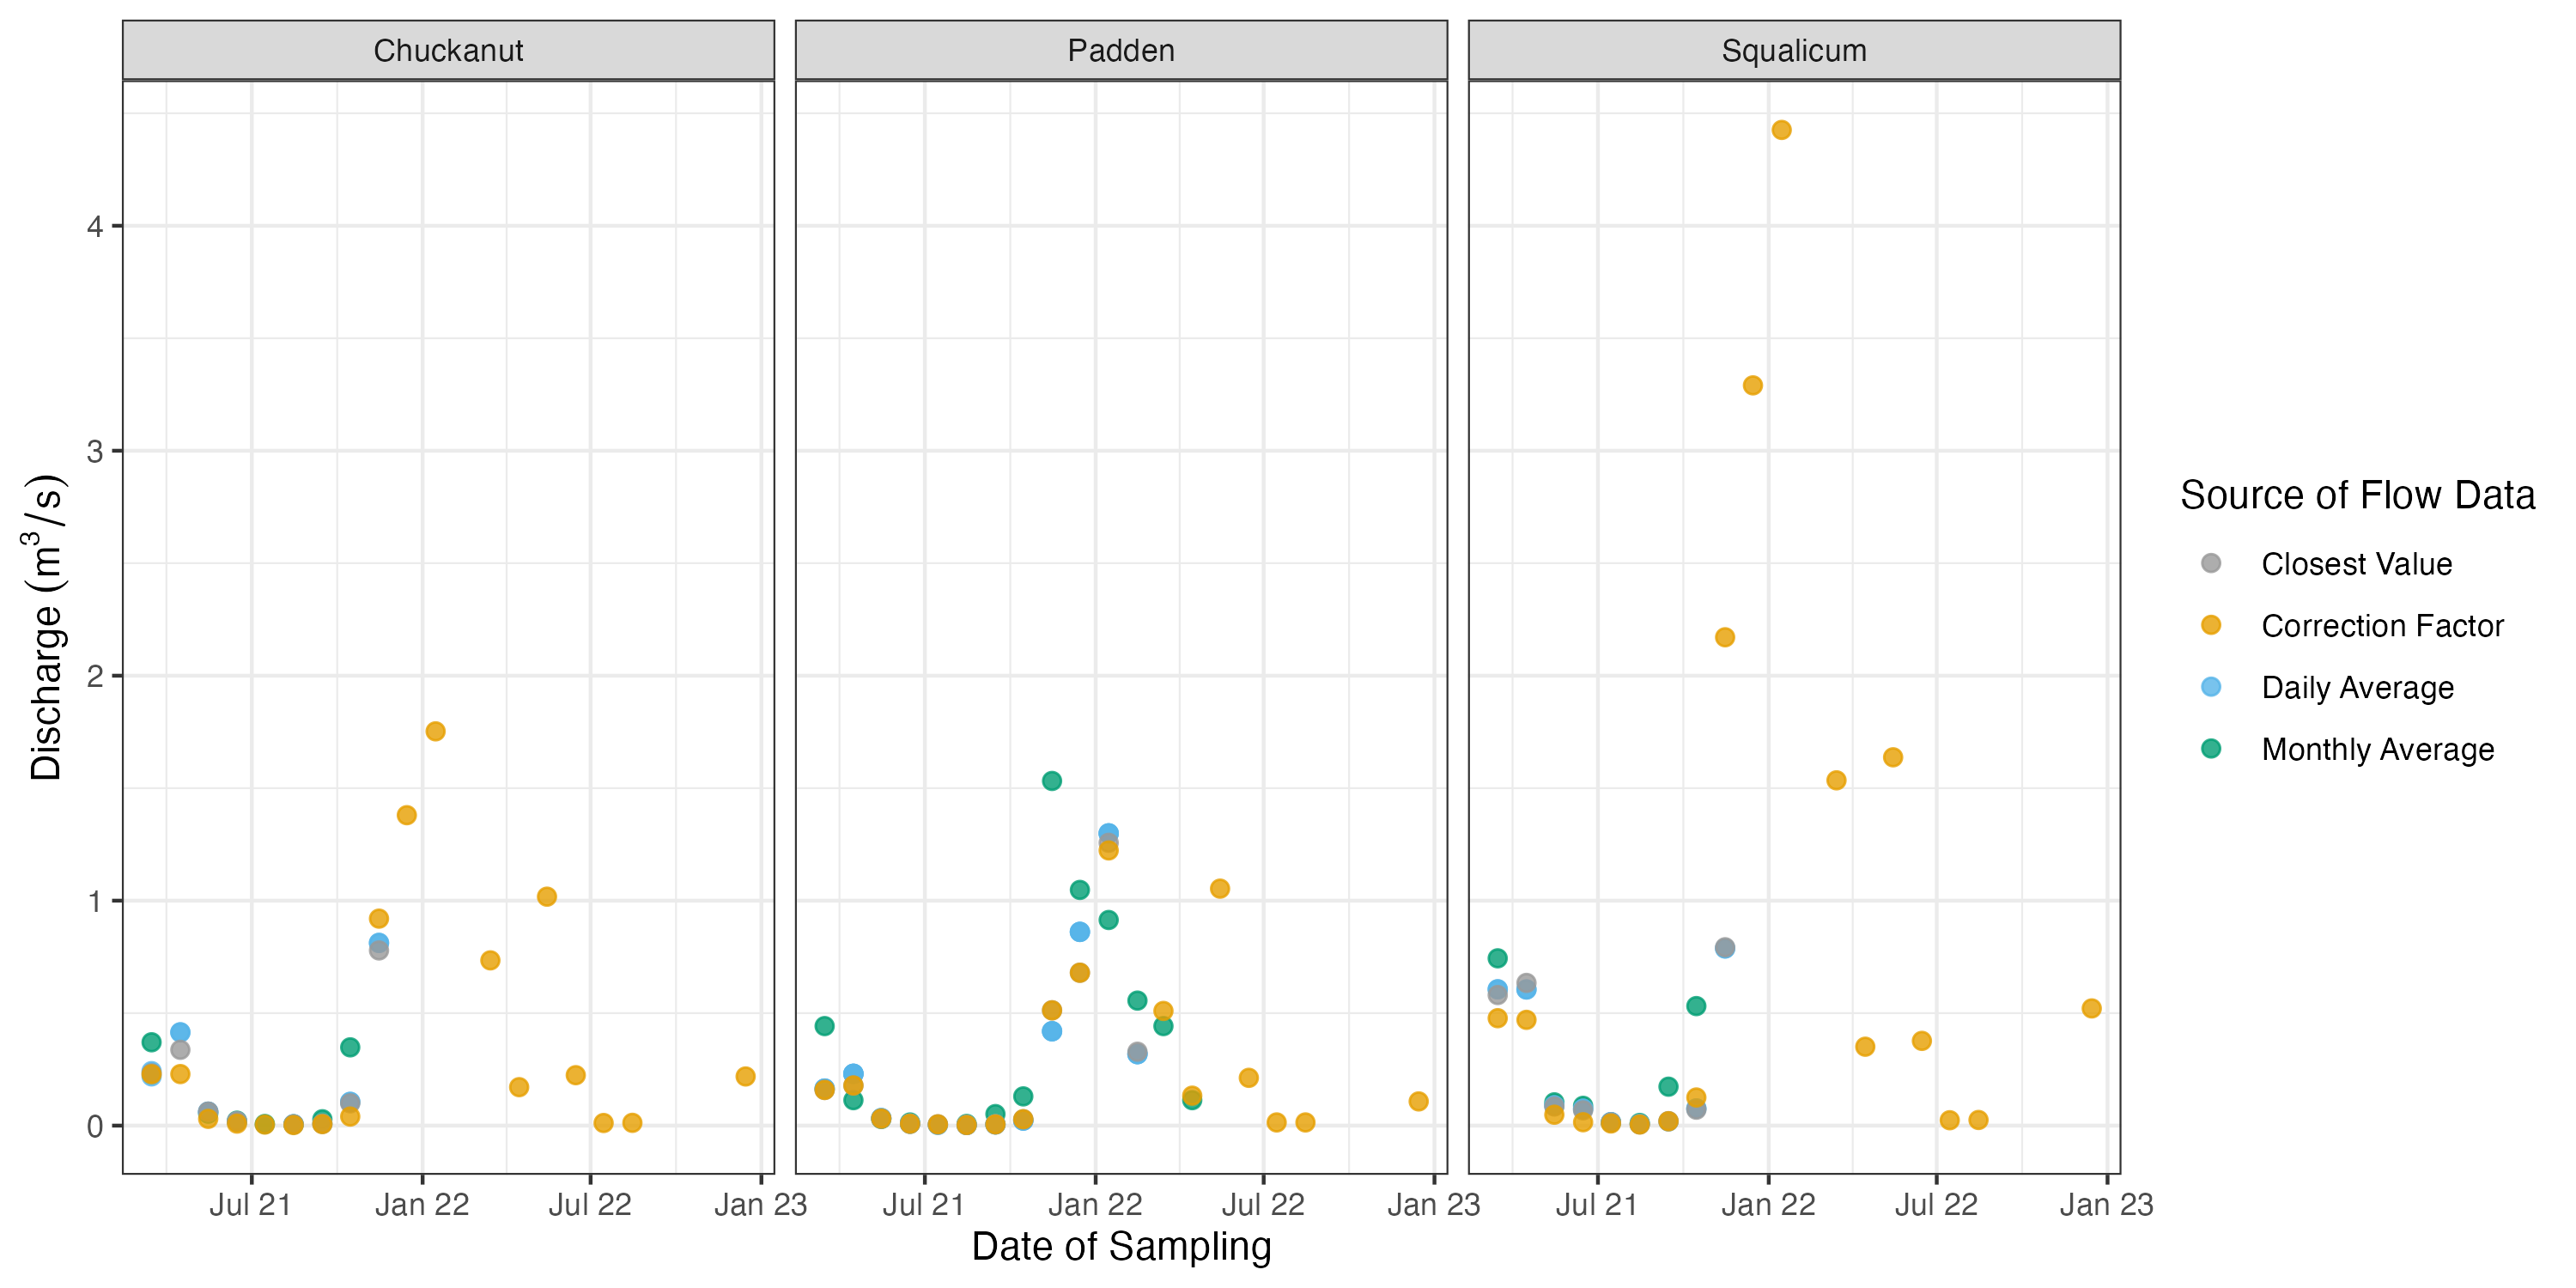
\includegraphics{../Output/SupplementalFigures/flow_by_source.png}
\caption{Figure S1.3. Comparison of different ways flow data can be used
to correct eDNA concentrations. In the main text, the correction factor
is used. Note that for Padden Creek, the ``Correction Factor'' method is
the same as the ``Closest Value'' method. Also note that for Chuckanut
and Squalicum Creeks, no data exist for cloest value, daily average, or
monthly average after November 2021 when the gauges went
offline.\label{fig:dischargemethod}}
\end{figure}

\hypertarget{construction-and-fish-exclusion}{%
\subsubsection{Construction and Fish
Exclusion}\label{construction-and-fish-exclusion}}

Fish were excluded from Padden Creek on August 30th, 2021 in preparation
for the stream to be diverted on September 9th, 2021 and the diversion
was removed October 7th, 2021. Water sampling occurred on September
10th, 2021, the day after the diversion, and on October 12, 2021, just 5
days after reconnecting the stream (Figure S1.\ref{fig:timeline}).

\hypertarget{stocking-in-lake-padden}{%
\subsubsection{Stocking in Lake Padden}\label{stocking-in-lake-padden}}

Padden Lake has historically been stocked with hatchery fish by the
Washington Department of Fish and Wildlife (Figure
S1.\ref{fig:timeline}). Rainbow trout (\emph{O. mykiss}) and
occassionally cutthroat trout (\emph{O. clarkii}) and kokanee salmon
(\emph{O. nerka}) are stocked in Lake Padden, approximately 1.5 km
upstream of the sampling sites. During the course of the study, rainbow
trout were stocked in April 2021 and April 2022, kokanee salmon were
stocked in May 2021 and October 2022, and cutthroat trout were stocked
in November 2022 (Figure S1.\ref{fig:timeline}). However, despite the
stocking of 30,000 kokanee salmon in May in Lake Padden, O. nerka was
not detected by metabarcoding in May 2021 or at any point in 2021 until
November (see main text Results). Importantly, this suggests that Lake
Padden is far enough upstream that the eDNA signal at the sampling sites
by the culvert is not a result of stocking the lake 1.5 km upstream (see
main text Discussion for more information).

\begin{figure}
\centering
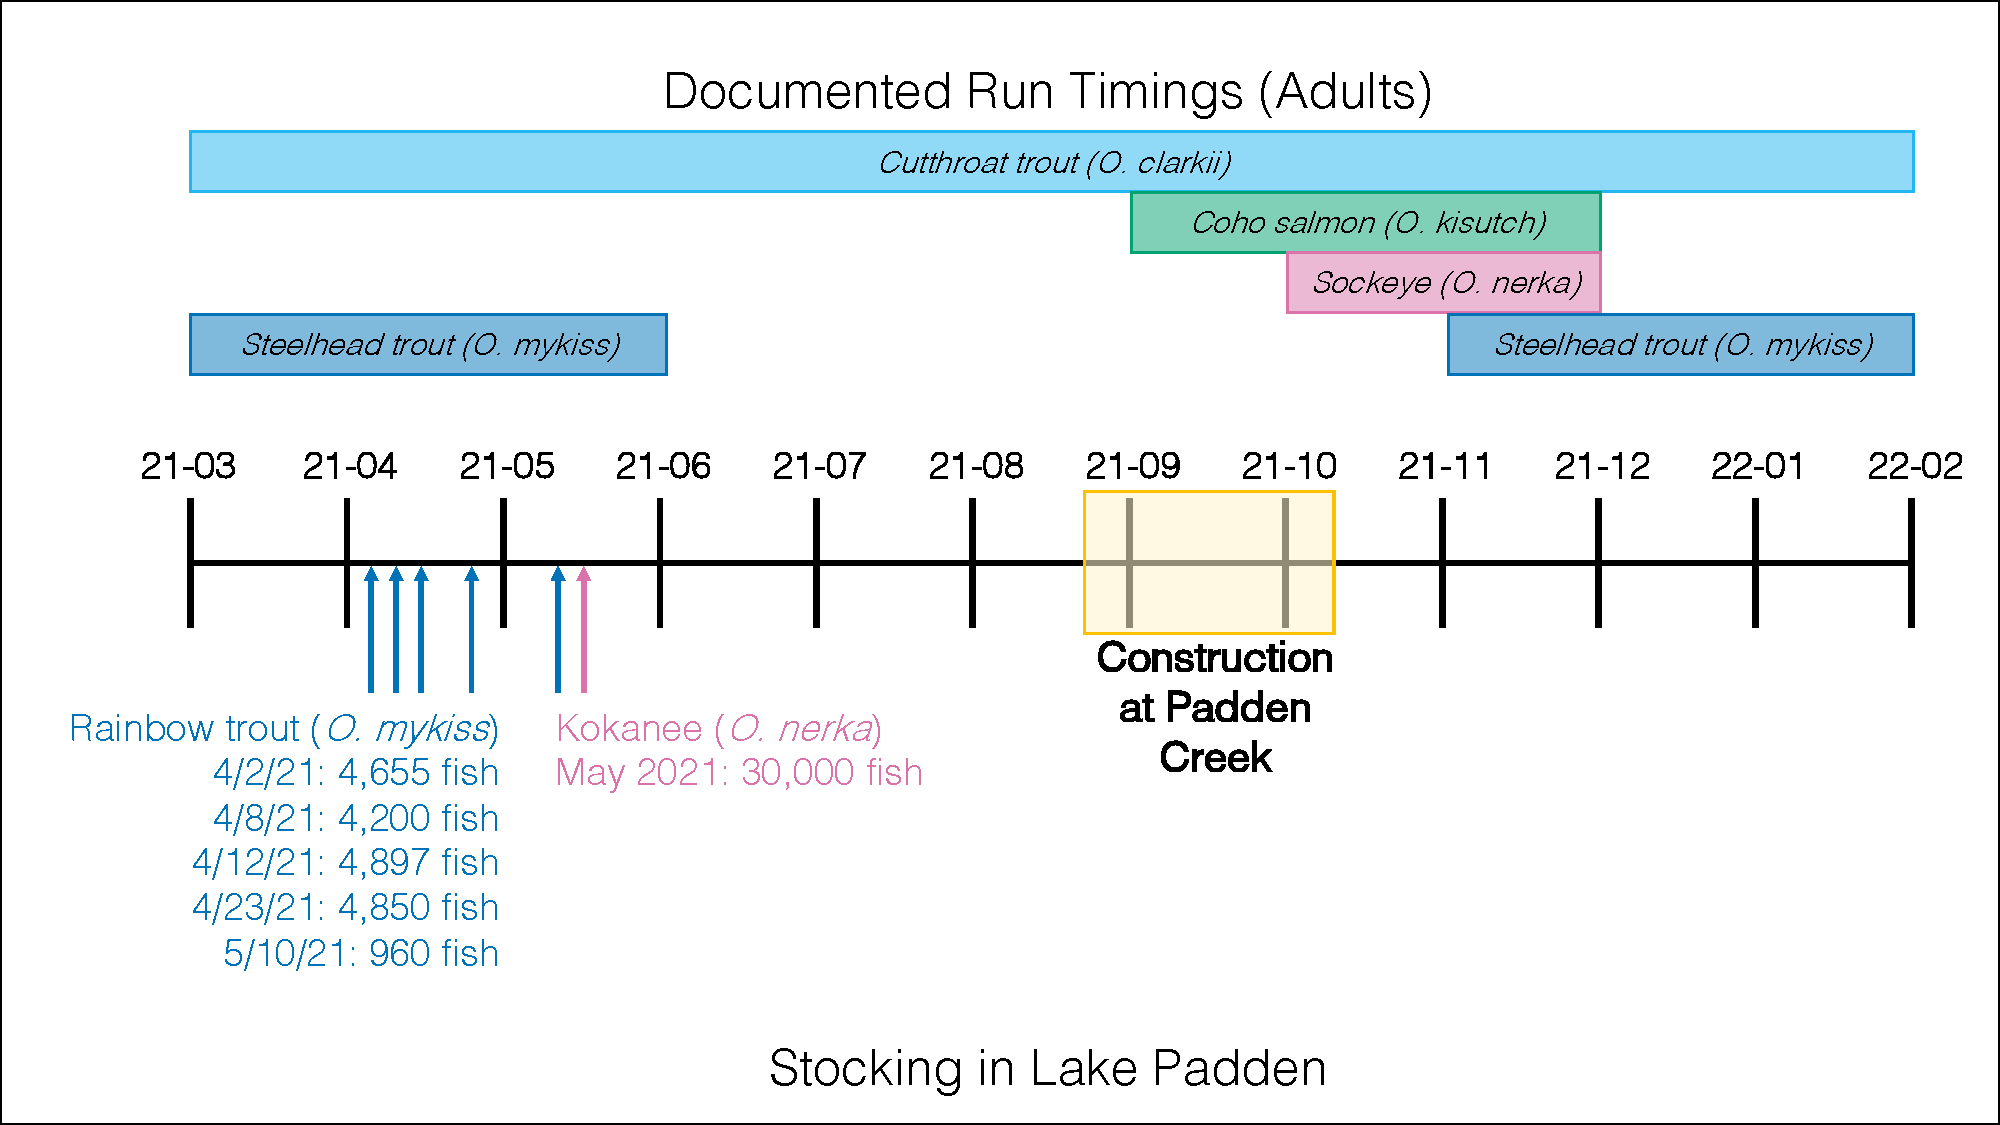
\includegraphics{../Output/SupplementalFigures/TimeLine.pdf}
\caption{Figure S1.4. Timeline of runs for migrating species, stocking
of Lake Padden, and construction at the intervention site (Padden
Creek). Note, the dates of kokanee stocking do not include days, just
the month and year. For plotting purposes, they are shown as the
15th.\label{fig:timeline}}
\end{figure}

\hypertarget{water-sampling}{%
\subsubsection{Water Sampling}\label{water-sampling}}

Water samples were collected using Smith Root's eDNA Backpack (Thomas et
al. 2018), a portable pumping-and-filtering setup set to filter at 1
L/min at 82.7 kPa (12 psi). For most months, a trident sampler was used
to collect all 3 biological replicates at the exact same time, for a
total sampling time of about 5 minutes. Otherwise, the three replicates
were collected consecutively, for a total sampling time of about 15
minutes. Downstream sites were always sampled before upstream sites to
ensure no potential DNA was introduced into the stream before sampling.
In some samples, less than 2 L of water was filtered due to clogging
(mean = 1.95 L).

\hypertarget{laboratory-processing}{%
\subsection{Laboratory Processing}\label{laboratory-processing}}

\hypertarget{dna-extraction-amplification-sequencing}{%
\subsubsection{DNA Extraction, Amplification,
Sequencing}\label{dna-extraction-amplification-sequencing}}

Here, we used mock communities to determine the species-specific
amplification efficiencies for each salmonid in the study. Briefly, we
constructed five communities with known proportions of starting DNA from
different species (total DNA as measured by Qubit). The communities
ranged from having a total of 12 to 20 species, but six salmonid species
were included in all five mock communities to have more information on
the amplification efficiencies of salmonids (Supplemental Table 2). We
sequenced these communities using the same metabarcoding primers and
thermocycling conditions above and then determined the species-specific
amplification rates given the discrepancy between the known starting
proportion and the proportion of reads after sequencing. The mock
community data were then used to correct the sequencing reads from the
environmental samples to estimate the starting DNA proportions of each
species in environmental samples, which is the metric of interest
(Figure 3, green boxes). This is the first application of the model to
correct eDNA data from water samples with mock community data as
described in Shelton et al. (2022) (see Supplemental Text 2 for more
information).

All molecular work prior to sequencing was performed at the University
of Washington. Bench-tops were cleaned with 10\% bleach for 10 minutes
and then wiped with 70\% ethanol. Molecular work was separated onto pre-
and post-PCR benches; all DNA extractions and PCR preparation was
conducted on a bench where no PCR product was handled.

\hypertarget{dna-extractions}{%
\subsubsection{DNA Extractions}\label{dna-extractions}}

We followed a protocol developed for extracting DNA off the
self-preserving Smith Root filters (Thomas et al. 2019). Filters were
removed from their housing with sterile tweezers and cut in half using
sterile razor blades. One half was archived and the other half was used
for extraction. DNA was extracted from half of each filter using a
Qiashredder column (Qiagen, USA) and the DNeasy Blood and Tissue Kit
(Qiagen, USA) with an overnight incubation (Thomas et al. (2019)), such
that the effective filtering effort was 1 L/sample; the remaining half
of each filter was archived at -20\degree C. Extracts were eluted in 100
\(\mu\)L of molecular grade water, quantified via Qubit (Invitrogen,
USA) and stored at -20\degree C until PCR amplification within 2 months
of extraction.

\hypertarget{pcr-amplification}{%
\subsubsection{PCR Amplification}\label{pcr-amplification}}

For the metabarcoding approach, we targeted a \textasciitilde186 bp
hypervariable region of the mitochondrial DNA 12S rRNA gene for PCR
amplification (MiFish; Miya et al.~2015), but using modified primer
sequences as given in Praebel and Wangensteen (unpublished; via personal
communication) and including the Illumina Nextera overhang sequences for
subsequent indexing. The primers used were as follows: F 5'
\emph{TCGTCGGCAGCGTCAGATGTGTATAAGAGACAG}GCCGGTAAAACTCGTGCCAGC 3', R 5'
\emph{GTCTCGTGGGCTCGGAGATGTGTATAAGAGACAG}CATAGTGGGGTATCTAATCCCAGTTTG 3'
(\emph{italics} indicate Nextera overhang). PCR reactions included 10
\(\mu\)L of 5X Platinum ii Buffer, 0.4 \(\mu\)L of Platinum ii Taq, 1.25
\(\mu\)L of 8 mM dNTPS, 1.25 \(\mu\)L of 10 \(\mu\)M F primer, 1.25
\(\mu\)L of 10 \(\mu\)M R primer, 5 \(\mu\)L of template, and 30.85
\(\mu\)L of molecular grade water, for a total reaction volume of 50
\(\mu\)L. Cycling conditions were as follows: 95\degree C for 2 min, 35
cycles of 95\degree C for 30 sec, 60\degree C for 30 sec, 72\degree C
for 30 sec, followed by a final extension of 72\degree C for 5 min.

Each month of samples was amplified on a single plate with the addition
of a no template control (NTC; molecular grade water in lieu of
template) and a positive control (genomic DNA from kangaroo). After PCR
amplification, PCR products were visualized on a 1-2\% gel. If no band
was present for a given sample, a new amplification was attempted with
extracts diluted 1:10 iteratively until a band was detected. PCR
products were size-selected and cleaned using MagBind Beads (Omega
Biotek, USA) at a sample:beads ratio of 1.2. Bead-cleaned PCR products
were eluted in 30 \(\mu\)L of molecular grade water and quantified via
Qubit (Invitrogen, USA).

An indexing PCR reaction added a unique index to each sample using
Nextera indices (Illumina, USA) to allow pooling multiple samples onto
the same sequencing run. For indexing, 10 ng of PCR product was used as
template in a final volume of 11.25 \(\mu\)L. For samples with
concentrations less than 0.88 ng/\(\mu\)L, 11.25 \(\mu\)L was added
despite being less than 10 ng of amplicon. Each sample received a unique
index; Nextera index sets A and B were used to avoid using the same
index for more than one sample on a single sequencing run. The PCR
reaction included the 11.25 \(\mu\)L of template, 12.5 \(\mu\)L of Kapa
HiFi MMX (Roche, USA), and 1.25 \(\mu\)L of indexed primer. Cycling
conditions were as follows: 95\degree C for 5 min, 8 cycles of
98\degree C for 20 sec, 56\degree C for 30 sec, 72\degree C for 3 min,
and a final extension of 72\degree C for 5 min.

Indexed PCR products were also size-selected and purified using MagBind
Beads (Omega Biotek, USA) at a sample:beads ratio of 0.8. Bead-cleaned
PCR products were eluted in 30 \(\mu\)L of molecular grade water and
quantified via Qubit. Indexed and bead-cleaned products were normalized
before pooling into libraries, which were subsequently quantified via
Qubit and visualized on a Bioanalyzer (Agilent, USA) before sequencing.
Samples were randomized in 3-month blocks and each block split across 3
sequencing runs, for a total of 12 sequencing runs. The loading
concentration of each library was 4-8 pM and 5-20\% PhiX was included
depending on the composition of the run. Sequencing was conducted using
an Illumina Miseq with v3 2x300 chemistry at the NOAA Northwest
Fisheries Science Center and the University of Washington's Northwest
Genomics Center.

\hypertarget{species-specific-qpcr}{%
\subsubsection{Species Specific qPCR}\label{species-specific-qpcr}}

We quantified cutthroat trout (\emph{O. clarkii}) DNA in each sample,
targeting a 114 bp fragment of the cytochrome b gene with a qPCR assay
(Duda et al. 2021). The primer/probe sequences were: F 5'
CCGCTACAGTCCTTCACCTTCTA 3', R 5' GATCTTTGTATGAGAAGTAAGGATGGAA 3', P 5'
6FAM-TGAGACAGGATCCAAC-MGB-NFQ 3'. The qPCR assay was multiplexed with
TaqMan Exogenous Internal Positive Control Reagents (EXO-IPC) (Applied
Biosystems, USA) to check for the presence of PCR inhibitors (Duda et
al. 2021). Each DNA sample was run in triplicate using Gene Expression
Mastermix (ThermoFisher, USA), a final concentration of 0.375 \(\mu\)M F
primer, 0.375 \(\mu\)M R primer, and 0.105 \(\mu\)M probe, as well as 1X
EXO-IPC mix, 1X EXO-IPC DNA, 3.5 \(\mu\)L of template for a final
reaction volume of 12 \(\mu\)L. The EXO-IPC mix includes the primers and
probe for the EXI-IPC DNA, with the probe having a VIC reporter,
allowing it to be multiplexed with the \emph{O. clarkii} assay, which
has a FAM reporter. All qPCRs were conducted on an Applied Biosystems
StepOnePlus thermocycler.

Thermocycling was as follows: 50\degree C for 2 min, 95\degree C for 10
min, followed by 45 cycles of 95\degree C for 15 sec, 60\degree C for 1
min. The cycle threshold (Ct) value determined for the EXO-IPC assay
from the NTC was compared to the Ct value for the EXO-IPC assay in each
of the environmental samples. If the Ct value was \textgreater0.5 Ct
values from the mean Ct for the NTCs, the sample was deemed inhibited
and diluted 1:10 and re-assayed until the Ct value fell within the
accepted range. After converting Ct values to DNA concentrations using
the standard curve (see below), the concentration was multiplied by the
dilution factor.

Each plate included a 8-point standard curve created using synthetic DNA
(gBlocks) at the following concentrations: 100,000 copies/\(\mu\)L,
10,000 copies/\(\mu\)L, 1,000 copies/\(\mu\)L, 100 copies/\(\mu\)L, 10
copies/\(\mu\)L, 5 copies/\(\mu\)L, 3 copies/\(\mu\)L, 1 copy/\(\mu\)L
Additionally, six no template controls (NTCs) were included on each
plate: 3 with the IPC DNA mix and 3 with molecular grade water instead
of template or IPC DNA mix. Plates were re-run if efficiency as
determined by the standard curve was outside of the range of 90-110\%.

To check for inhibition, the cycle threshold (Ct) value determined for
the EXO-IPC assay from the NTC was compared to the Ct value for the
EXO-IPC assay in each of the environmental samples. If the Ct value was
\textgreater0.5 Ct values from the mean Ct for the NTCs, the sample was
deemed inhibited and diluted 1:10 and re-assayed until the Ct value fell
within the accepted range. The majority of environmental samples (60\%)
were inhibited and accordingly diluted for analysis. In 80\% of
inhibited samples, a 1:10 dilution or less remedied the inhibition, but
some samples (11\%) required dilution by a factor of up to 1000.

\hypertarget{bioinformatics-processing}{%
\subsection{Bioinformatics Processing}\label{bioinformatics-processing}}

Primers were removed with cutadapt (Martin 2011) and then reads were
de-noised, filtered, merged, and ASVs were generated using dada2
(Callahan et al. 2016). For each MiSeq run, the trimming lengths were
determined by visually assessing the quality score plots. After ASVs
were generated, taxonomy was assigned using the ``classify'' function in
the insect package in R using the classifier published by the authors of
the package (Wilkinson et al. 2018).

\hypertarget{quality-controls}{%
\subsubsection{Quality Controls}\label{quality-controls}}

Positive controls were included on each sequencing run to monitor for
cross contamination that might have occurred in the laboratory or due to
``tag jumping''. With 13 MiSeq runs, we included one sample of kangaroo
tissue on each run and then measured how many reads of kangaroo were
found in environmental samples and how many reads of non-kangaroo were
found in kangaroo samples (Figure S1.\ref{fig:controls1}).

\begin{figure}
\centering
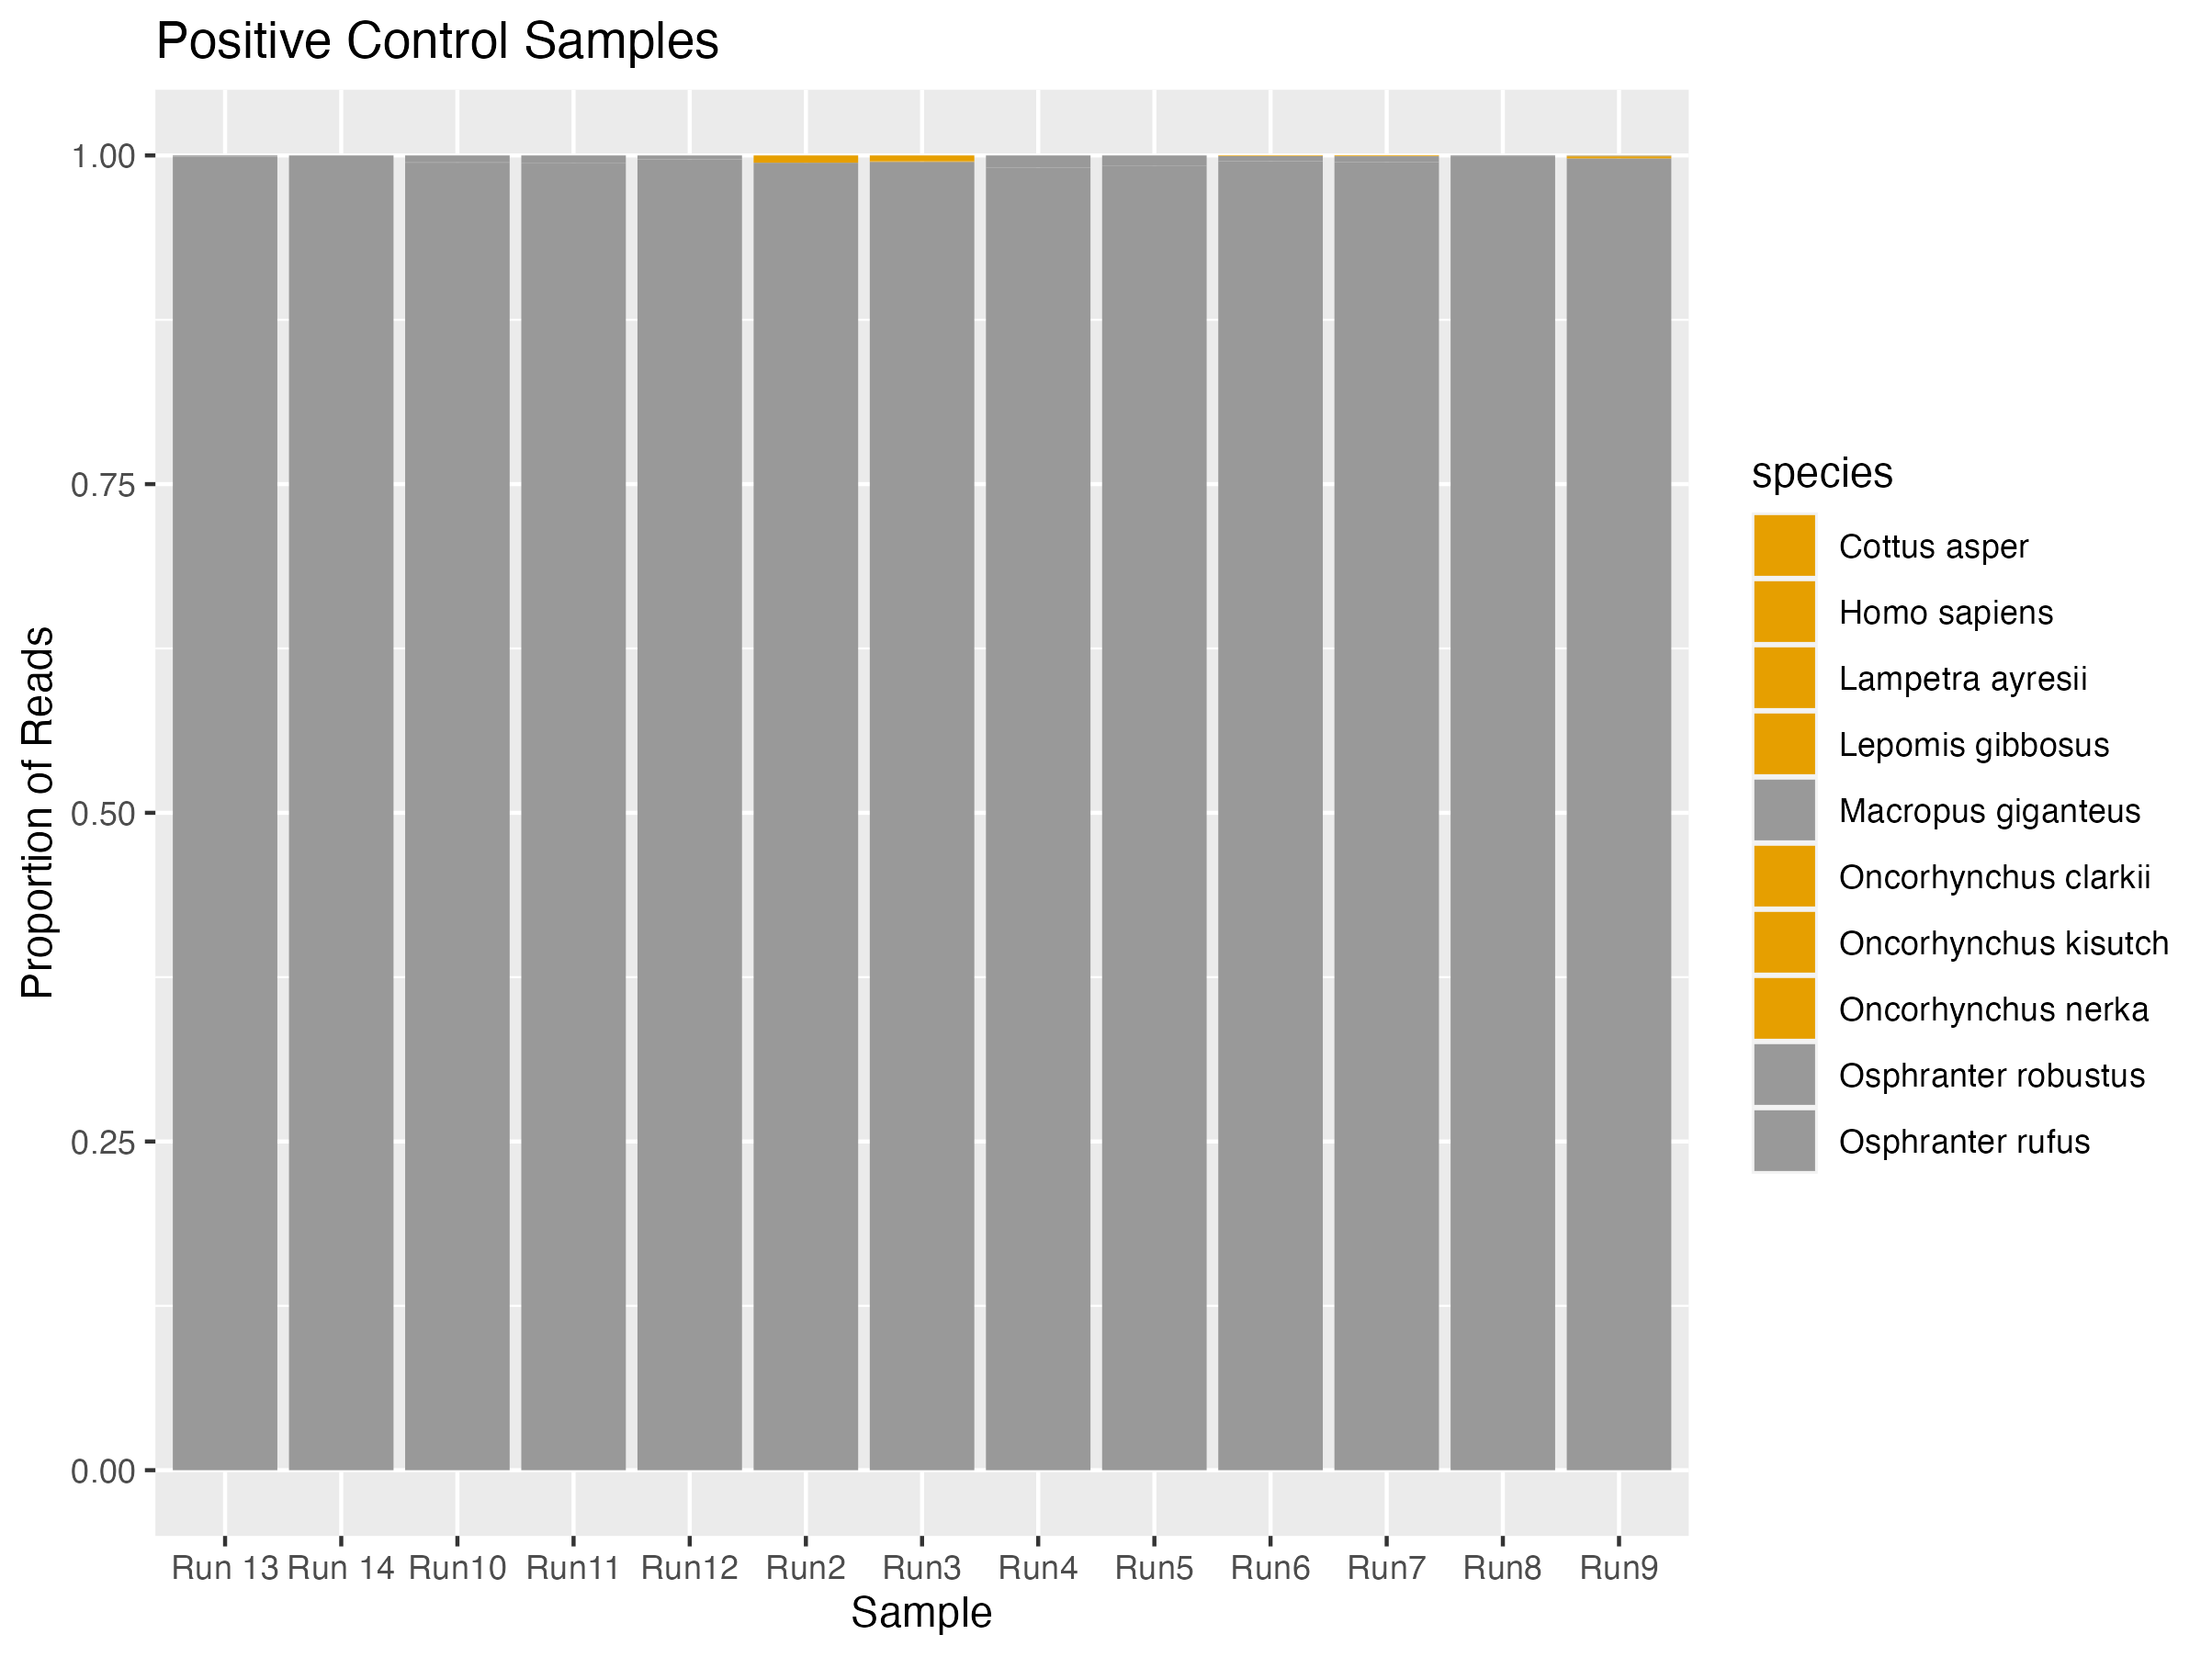
\includegraphics{../Output/SupplementalFigures/check_controls.png}
\caption{Figure S1.5. Proporiton of annotated reads found in positive
controls. Grey colors are the three species of kangaroo used for
positive controls and are what should be in each sample. Orange species
should not be in the positive controls and indicate low level
contamination from environmental samples.\label{fig:controls1}}
\end{figure}

We can also check to make sure that no reads assigning to kangaroo were
in the environmental samples. We only found kangaroo in two
environmental samples, both of which were a very small number (and
proportion) of reads (2 and 136 reads found in samples with 40,425 and
28,725 reads respectively) (Figure S1.\ref{fig:controls2}).

\begin{figure}
\centering
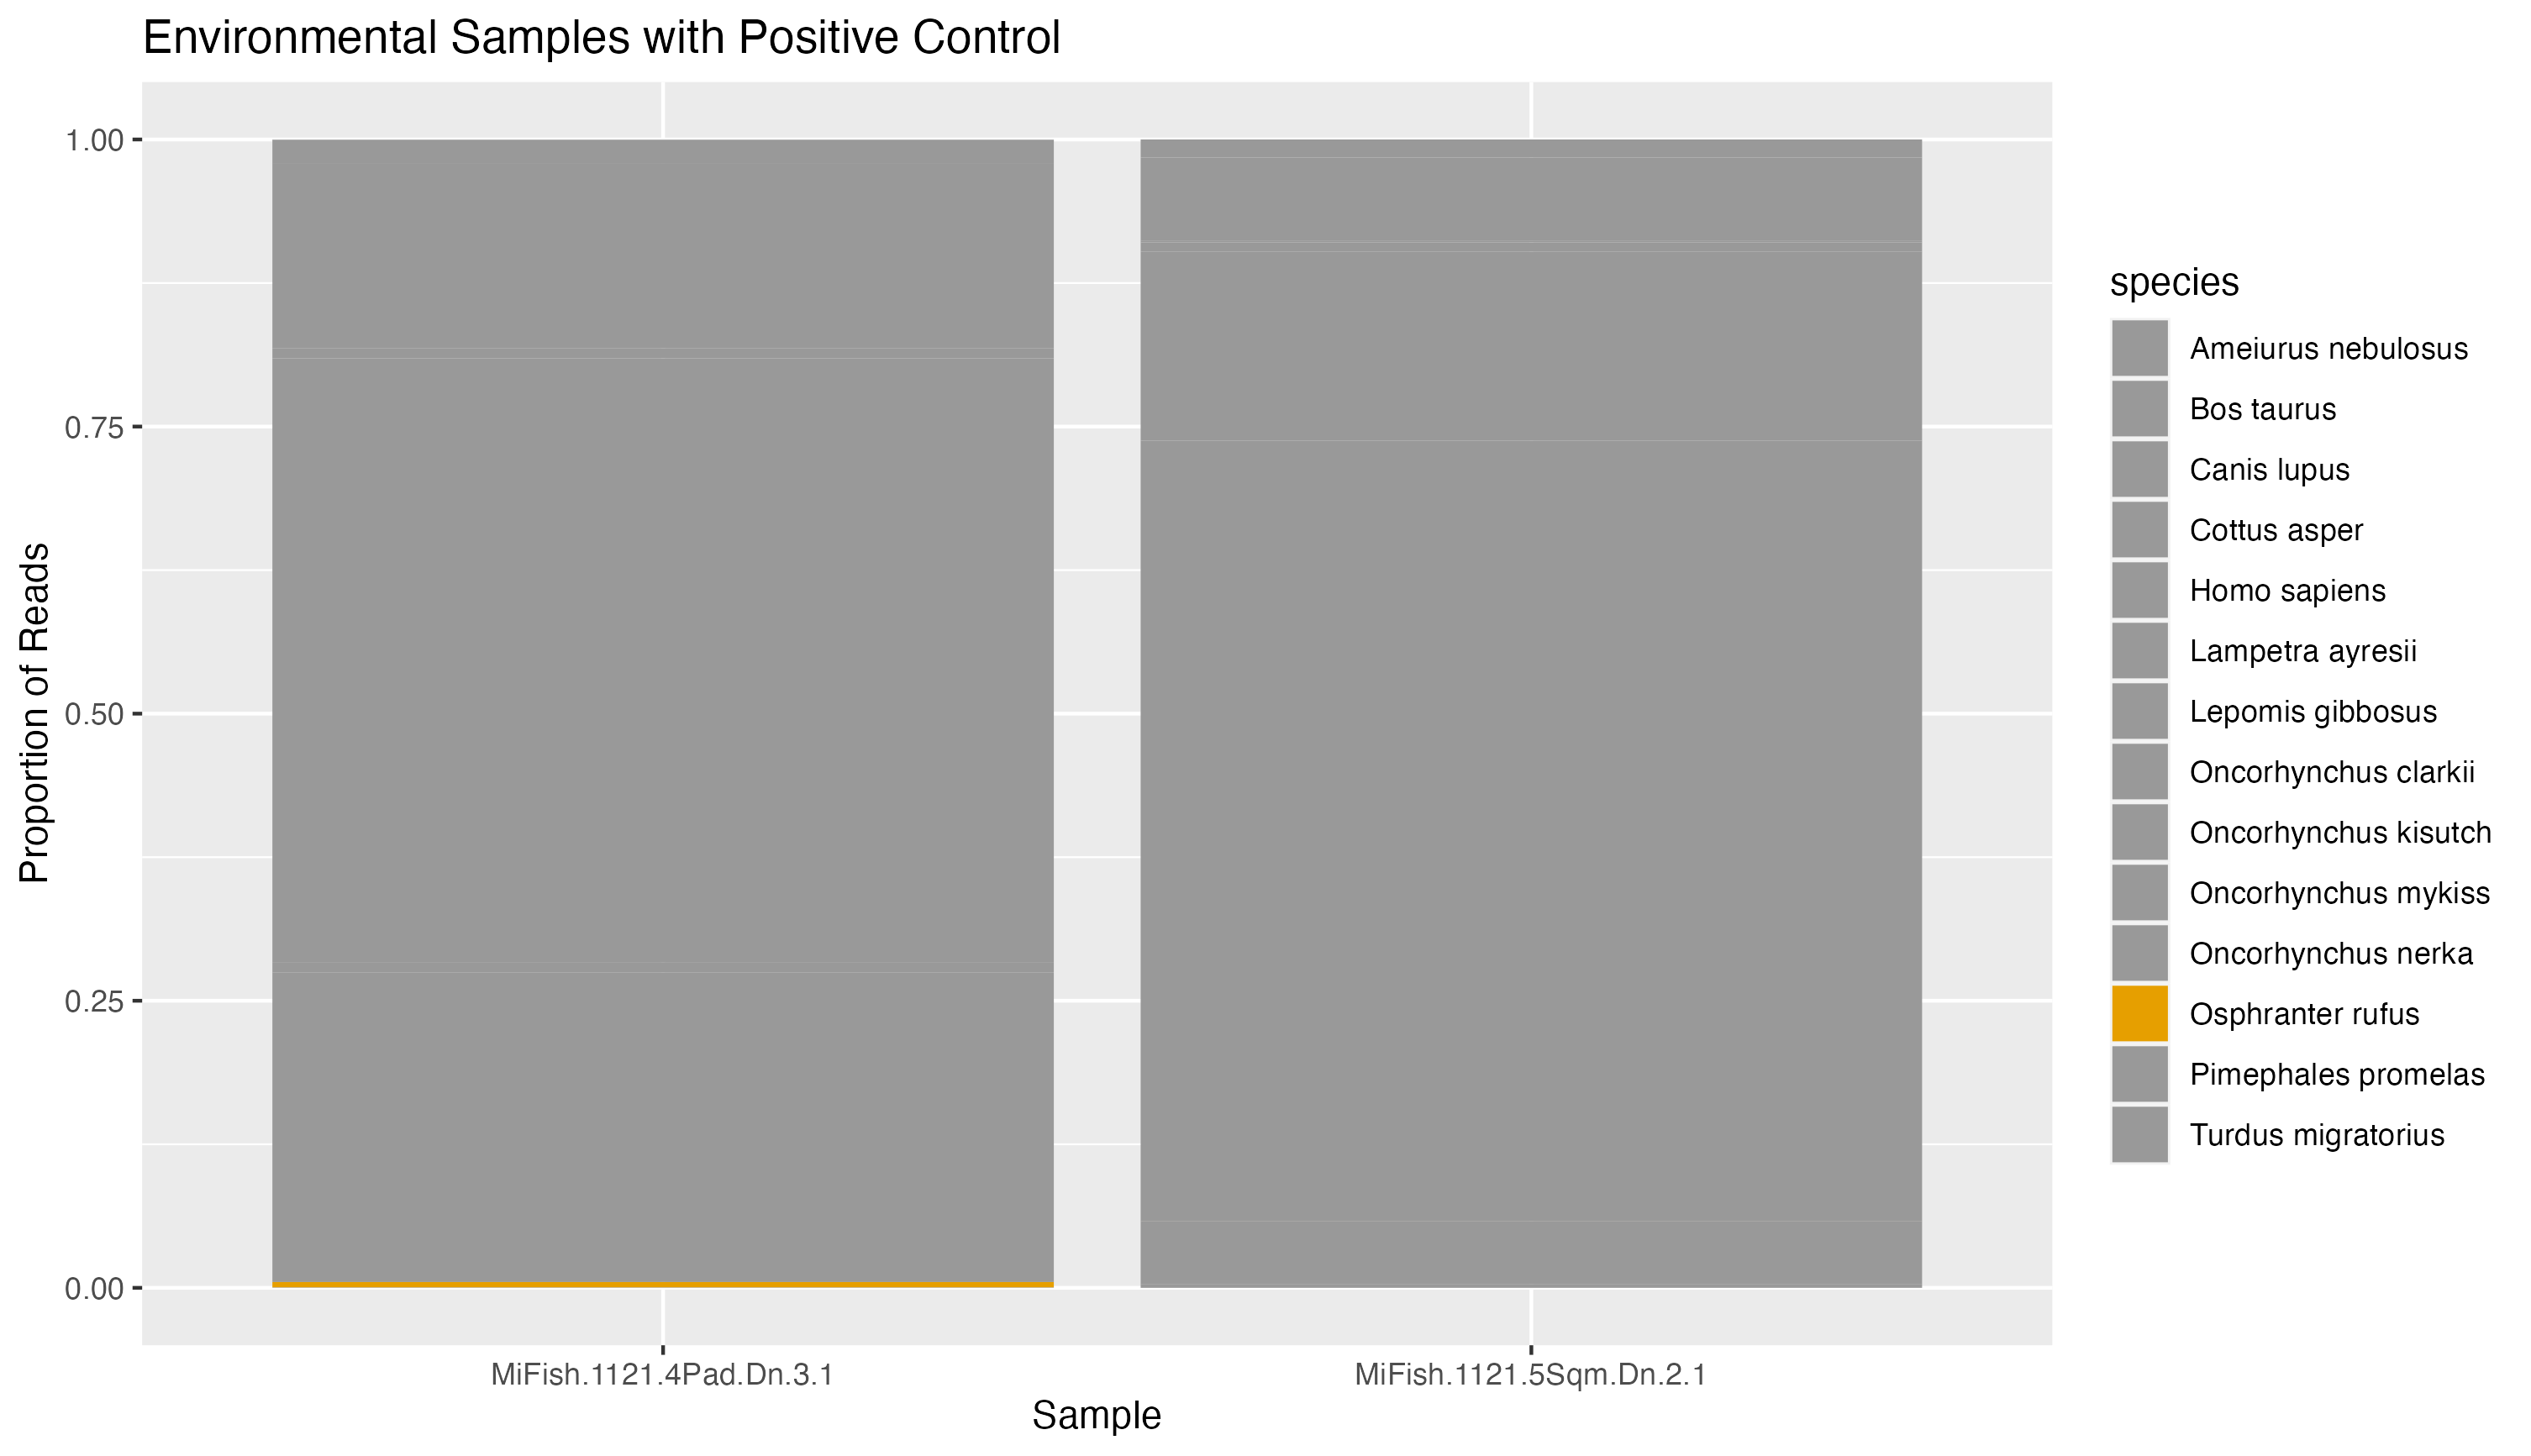
\includegraphics{../Output/SupplementalFigures/check_controls2.png}
\caption{Figure S1.6. Proporiton of annotated reads found in
environmental samples with positive control. Grey colors are
non-kangaroo reads and therefore and are what should be in each sample.
Orange species are kangaroo reads and therefore should not be in the
environmental samples and indicate low level contamination from positive
controls.\label{fig:controls2}}
\end{figure}

\hypertarget{annotation}{%
\subsubsection{Annotation}\label{annotation}}

We first used a tree-based annotation method (insect package) and then
followed up with a BLAST search for all ASVs that were not annotated to
species level by insect. The percent of reads annotated did not
correlate with sample read depth, creek, station, or month of sampling.
Read depth across samples ranged from 1,011 to 311,879, with a mean of
79,709 and median of 75,967 reads (Figure S1.\ref{fig:readdepth}). With
a total of \textasciitilde565 samples, 93\% of samples had
\textgreater20,000 reads and 65\% of samples had over 50,000 reads.
There did not seem to be a pattern with samples of low reads with creek
or time. Additionally, of the low read depth samples (\textless20,000
reads, 40 samples), there was only one sample in which all three
replicates were low (March 2022 Squalicum Upstream), meaning that it is
very unlikely that low read depth samples would have lead to changing
ecological results.

\begin{figure}
\centering
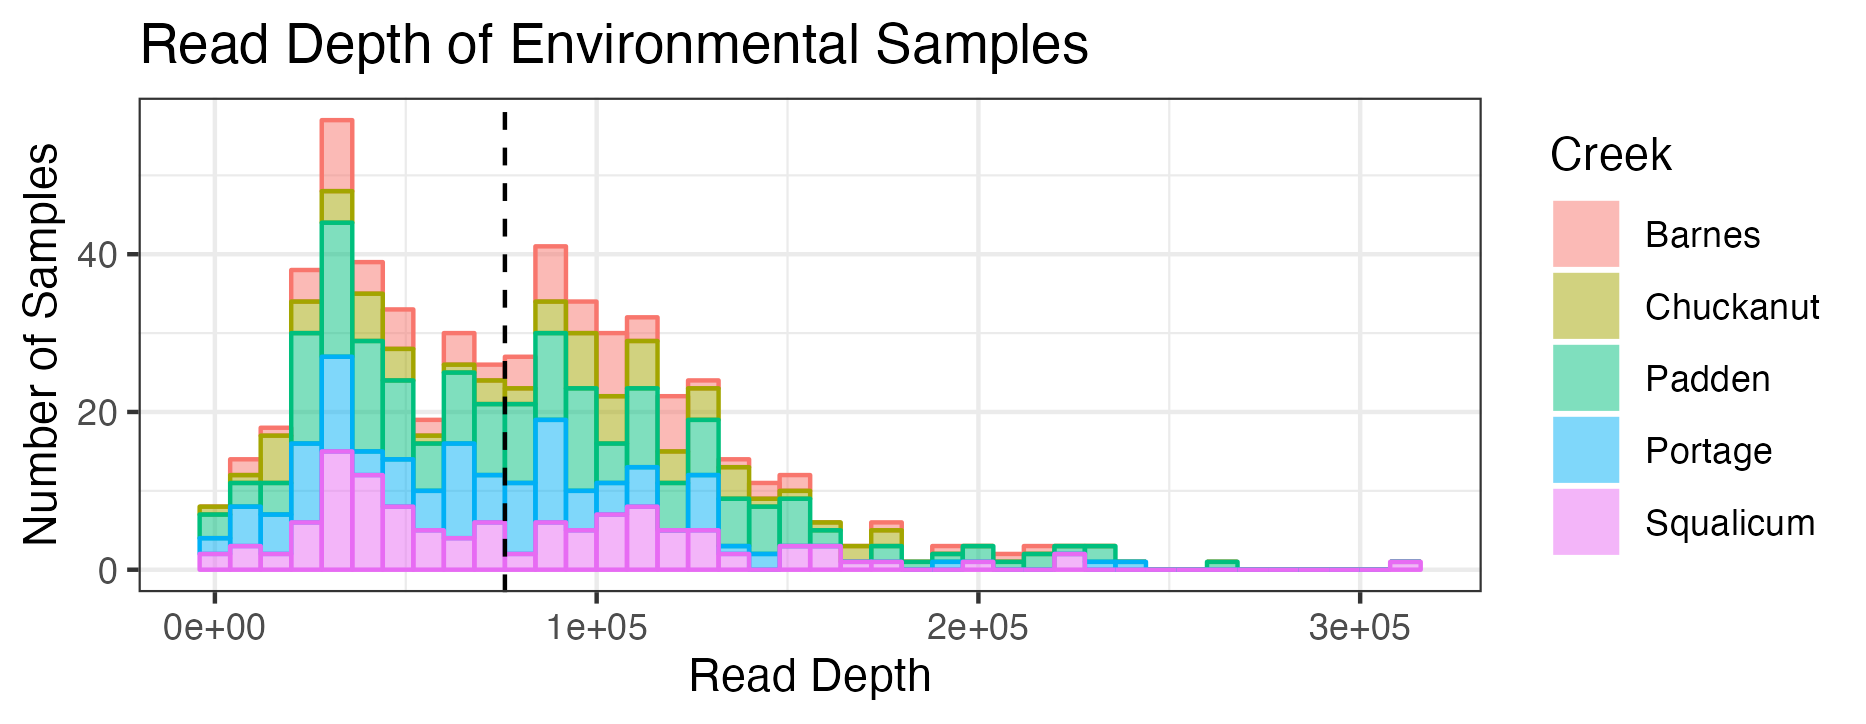
\includegraphics{../Output/SupplementalFigures/read_depths.png}
\caption{Figure S1.7. Read depth of samples colored by creek. Dashed
line shows median read depth (87,698 reads).\label{fig:readdepth}}
\end{figure}

A total of 81 unique species were identified in the environmental
samples by the MiFish primers, including 25 fish, 25 mammals, 23 birds ,
and 8 amphibians (Figure S1.\ref{fig:controlreads} and
S1.\ref{fig:paddenreads}; see also Supplemental Table 1). Of the 81
species, 17 only were found in a single environmental sample. The three
most commonly found species were coho salmon (\emph{O. kisutch}),
cutthroat trout (\emph{O. clarkii}), and rainbow trout (\emph{O.
mykiss}).

\begin{figure}
\centering
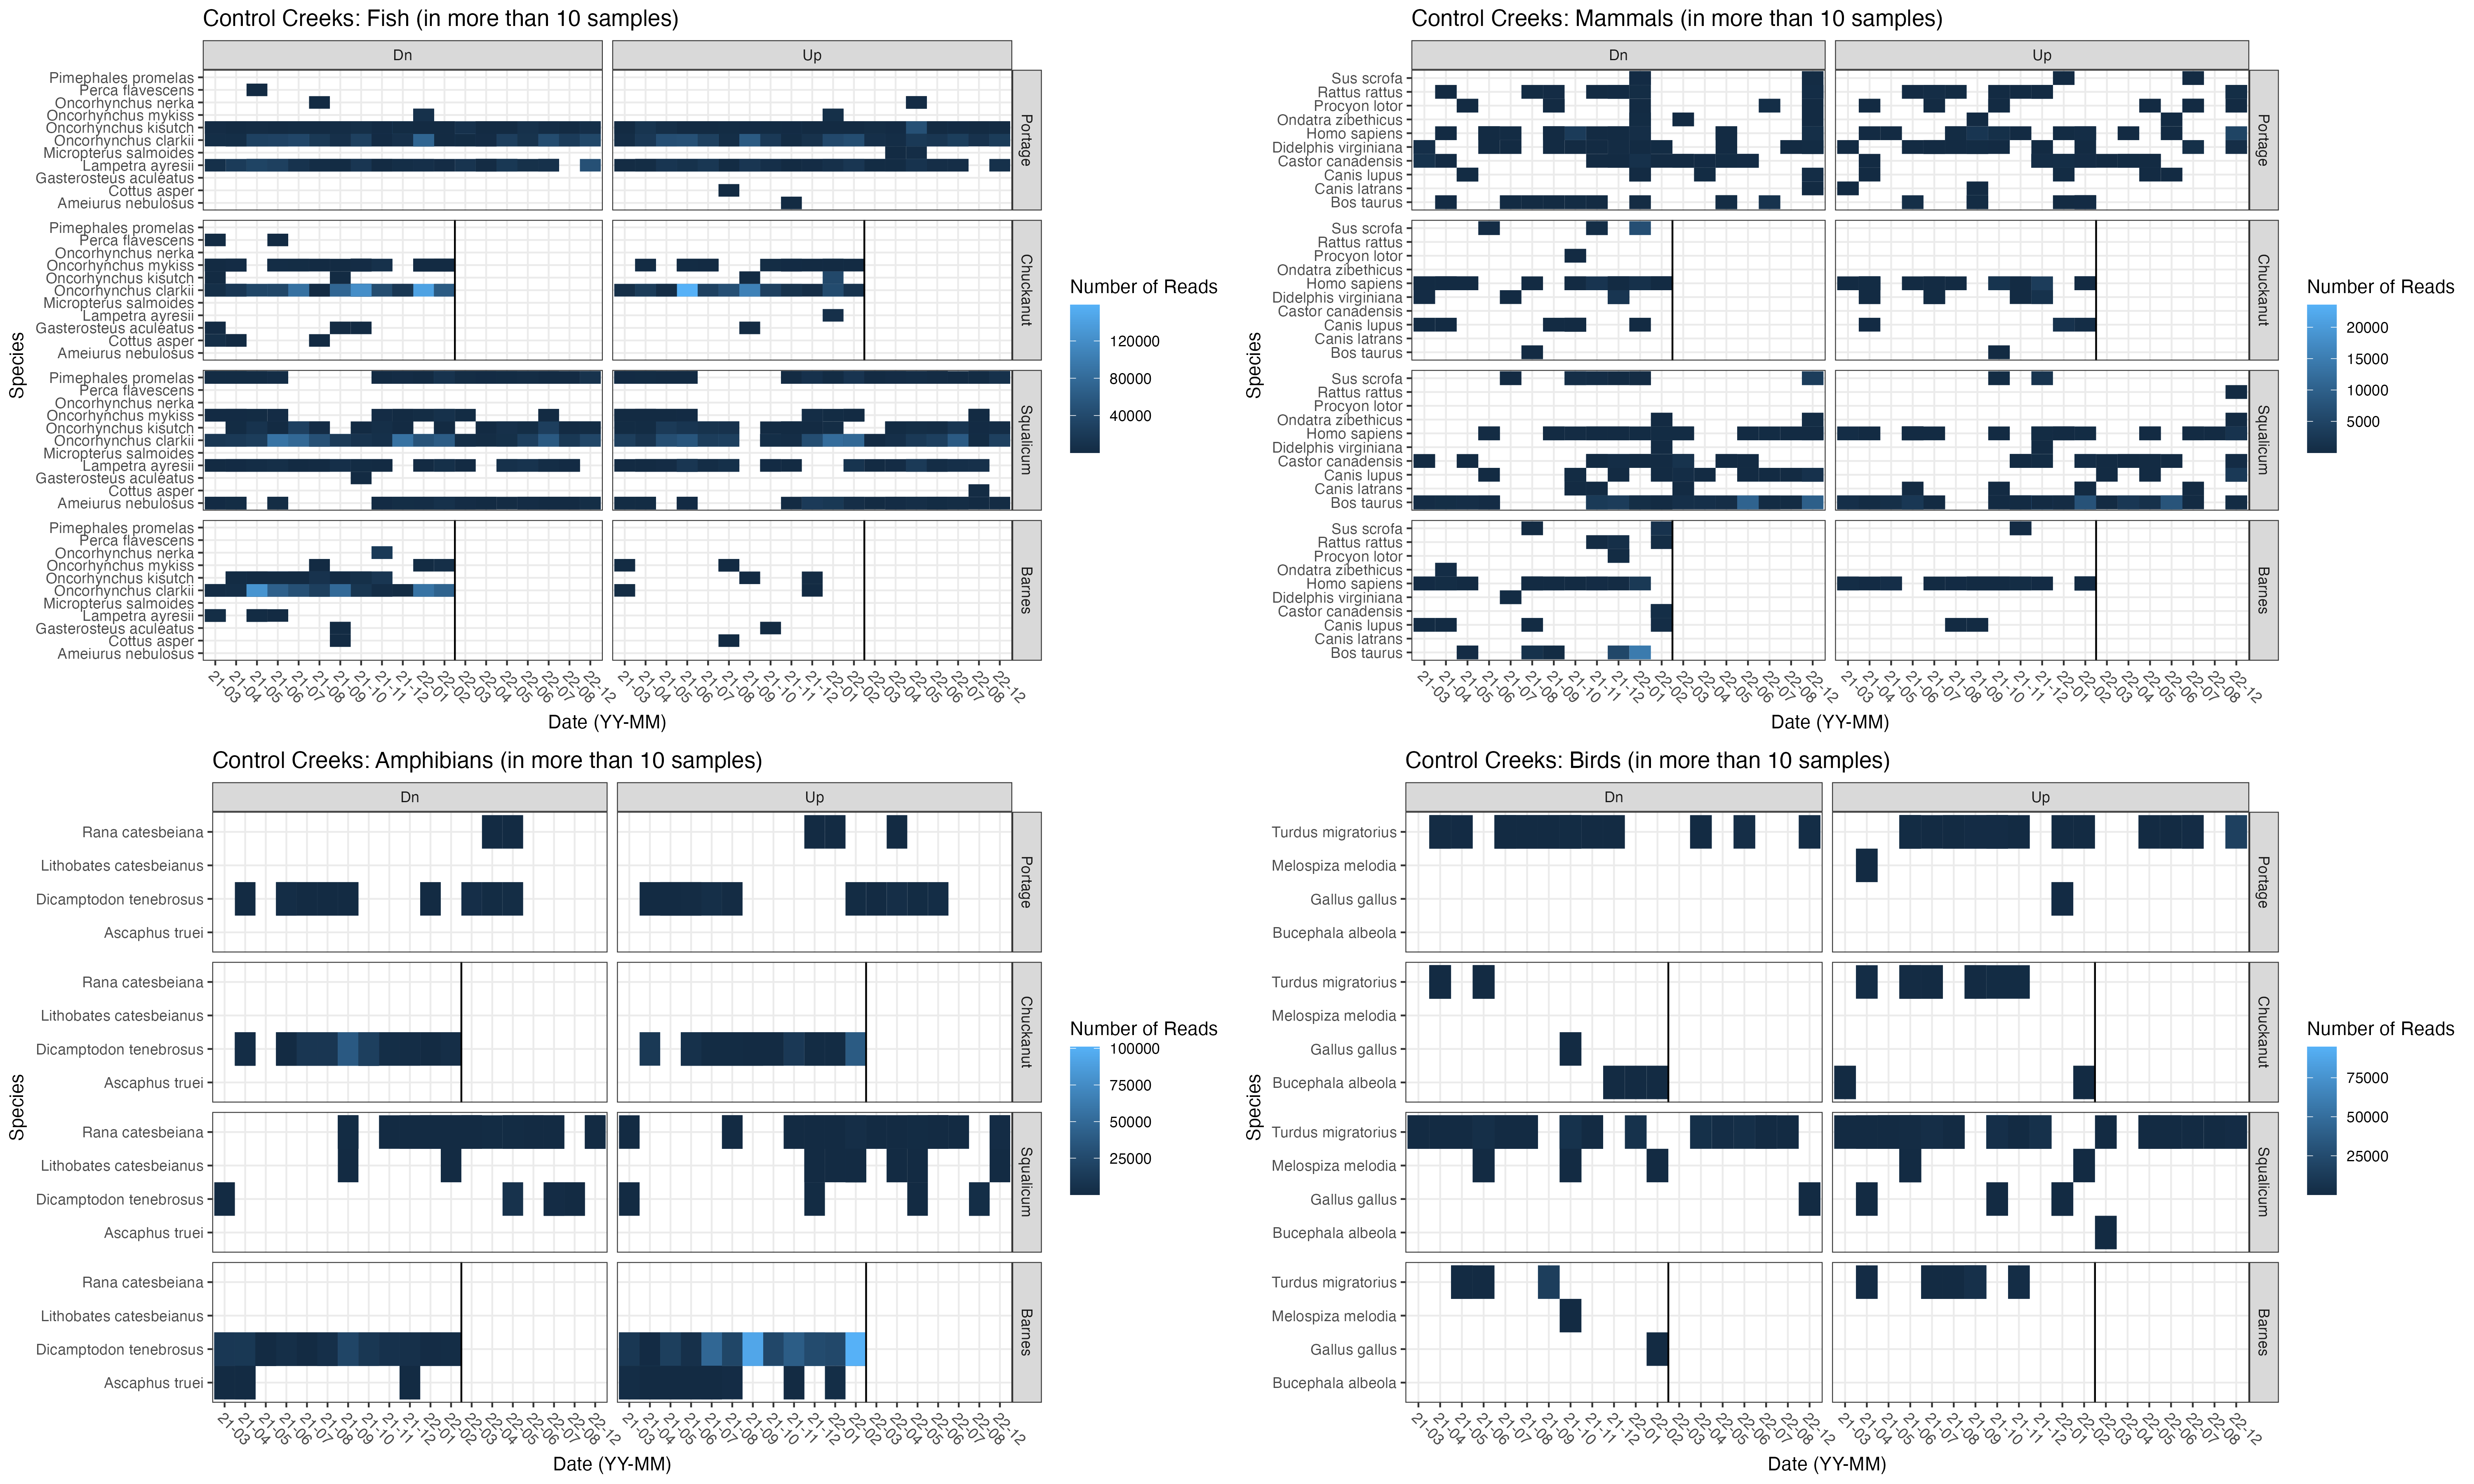
\includegraphics{../Output/SupplementalFigures/ALLTAXA_controls.png}
\caption{Figure S1.8. Heat map of all species found in control creeks in
at least ten environmental samples.\label{fig:controlreads}}
\end{figure}

\begin{figure}
\centering
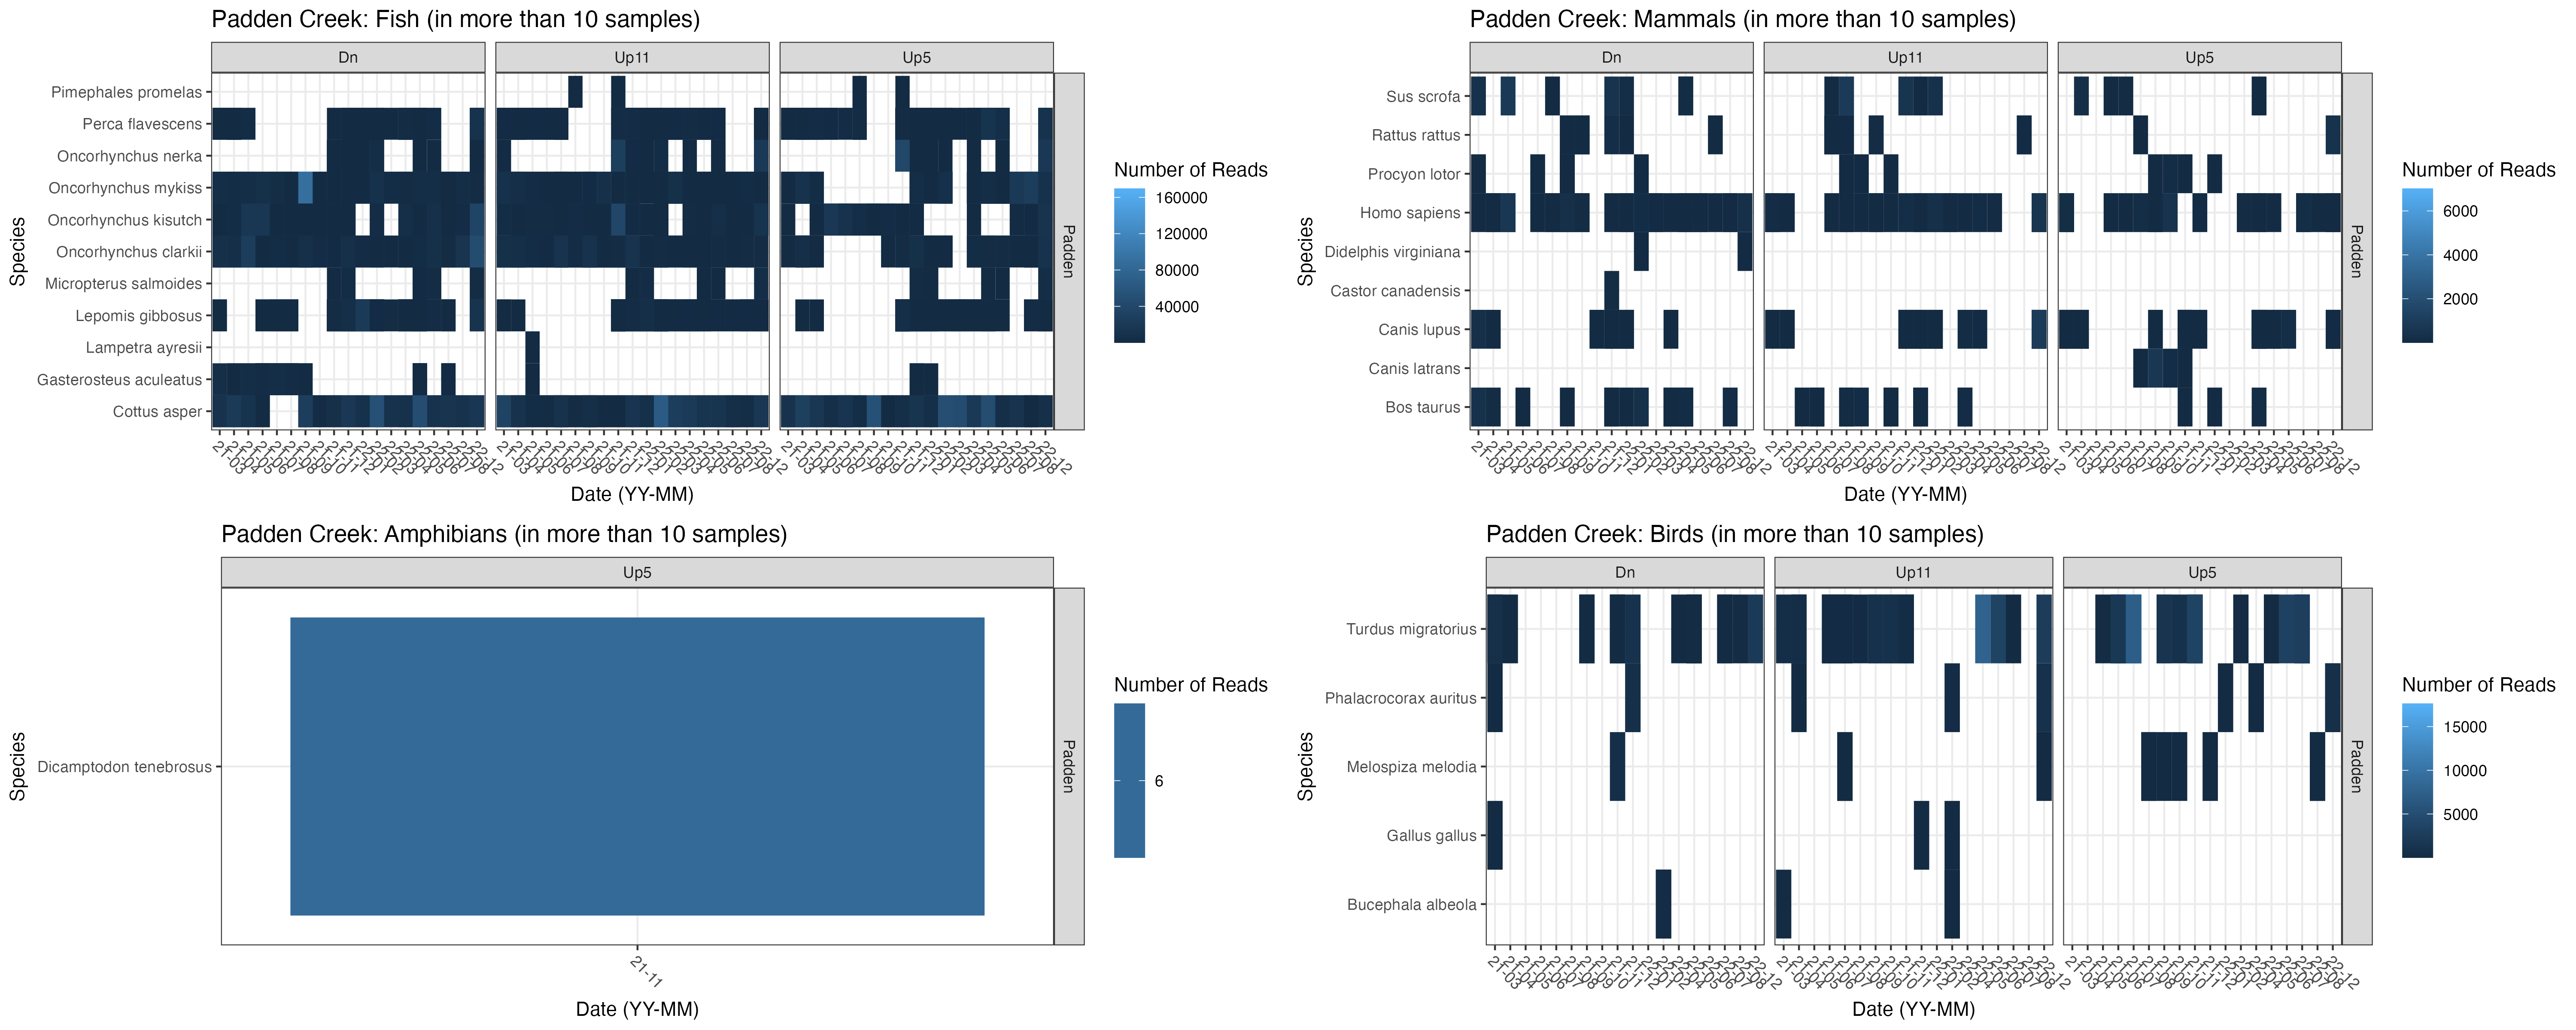
\includegraphics{../Output/SupplementalFigures/ALLTAXA_padden.png}
\caption{Figure S1.9. Heat map of all species found in Padden Creek in
at least ten environmental samples.\label{fig:paddenreads}}
\end{figure}

\hypertarget{correcting-metabarcoding-data-for-amplification-bias}{%
\subsection{Correcting metabarcoding data for amplification
bias}\label{correcting-metabarcoding-data-for-amplification-bias}}

Using our six mock communities (three different taxa compositions at two
different proportions {[}even and skewed{]}), we can first check how
well the quantitative metabarcoding model corrects for amplification
bias. In one case, we consider the even mock communities as the mock
community data and the skewed mock communities as unknown. We can then
re-create what the model believes to be the original starting
proportions of the skewed mock community given the proportions of reads
found in the skewed mock communities and the proportion of DNA as
compared to the proportion of reads found in the even mock communities.
We can also do the same treating the skewed mock communities as known
and even mock communities as unknown (Figure S1.\ref{fig:intercal}).

\begin{figure}
\centering
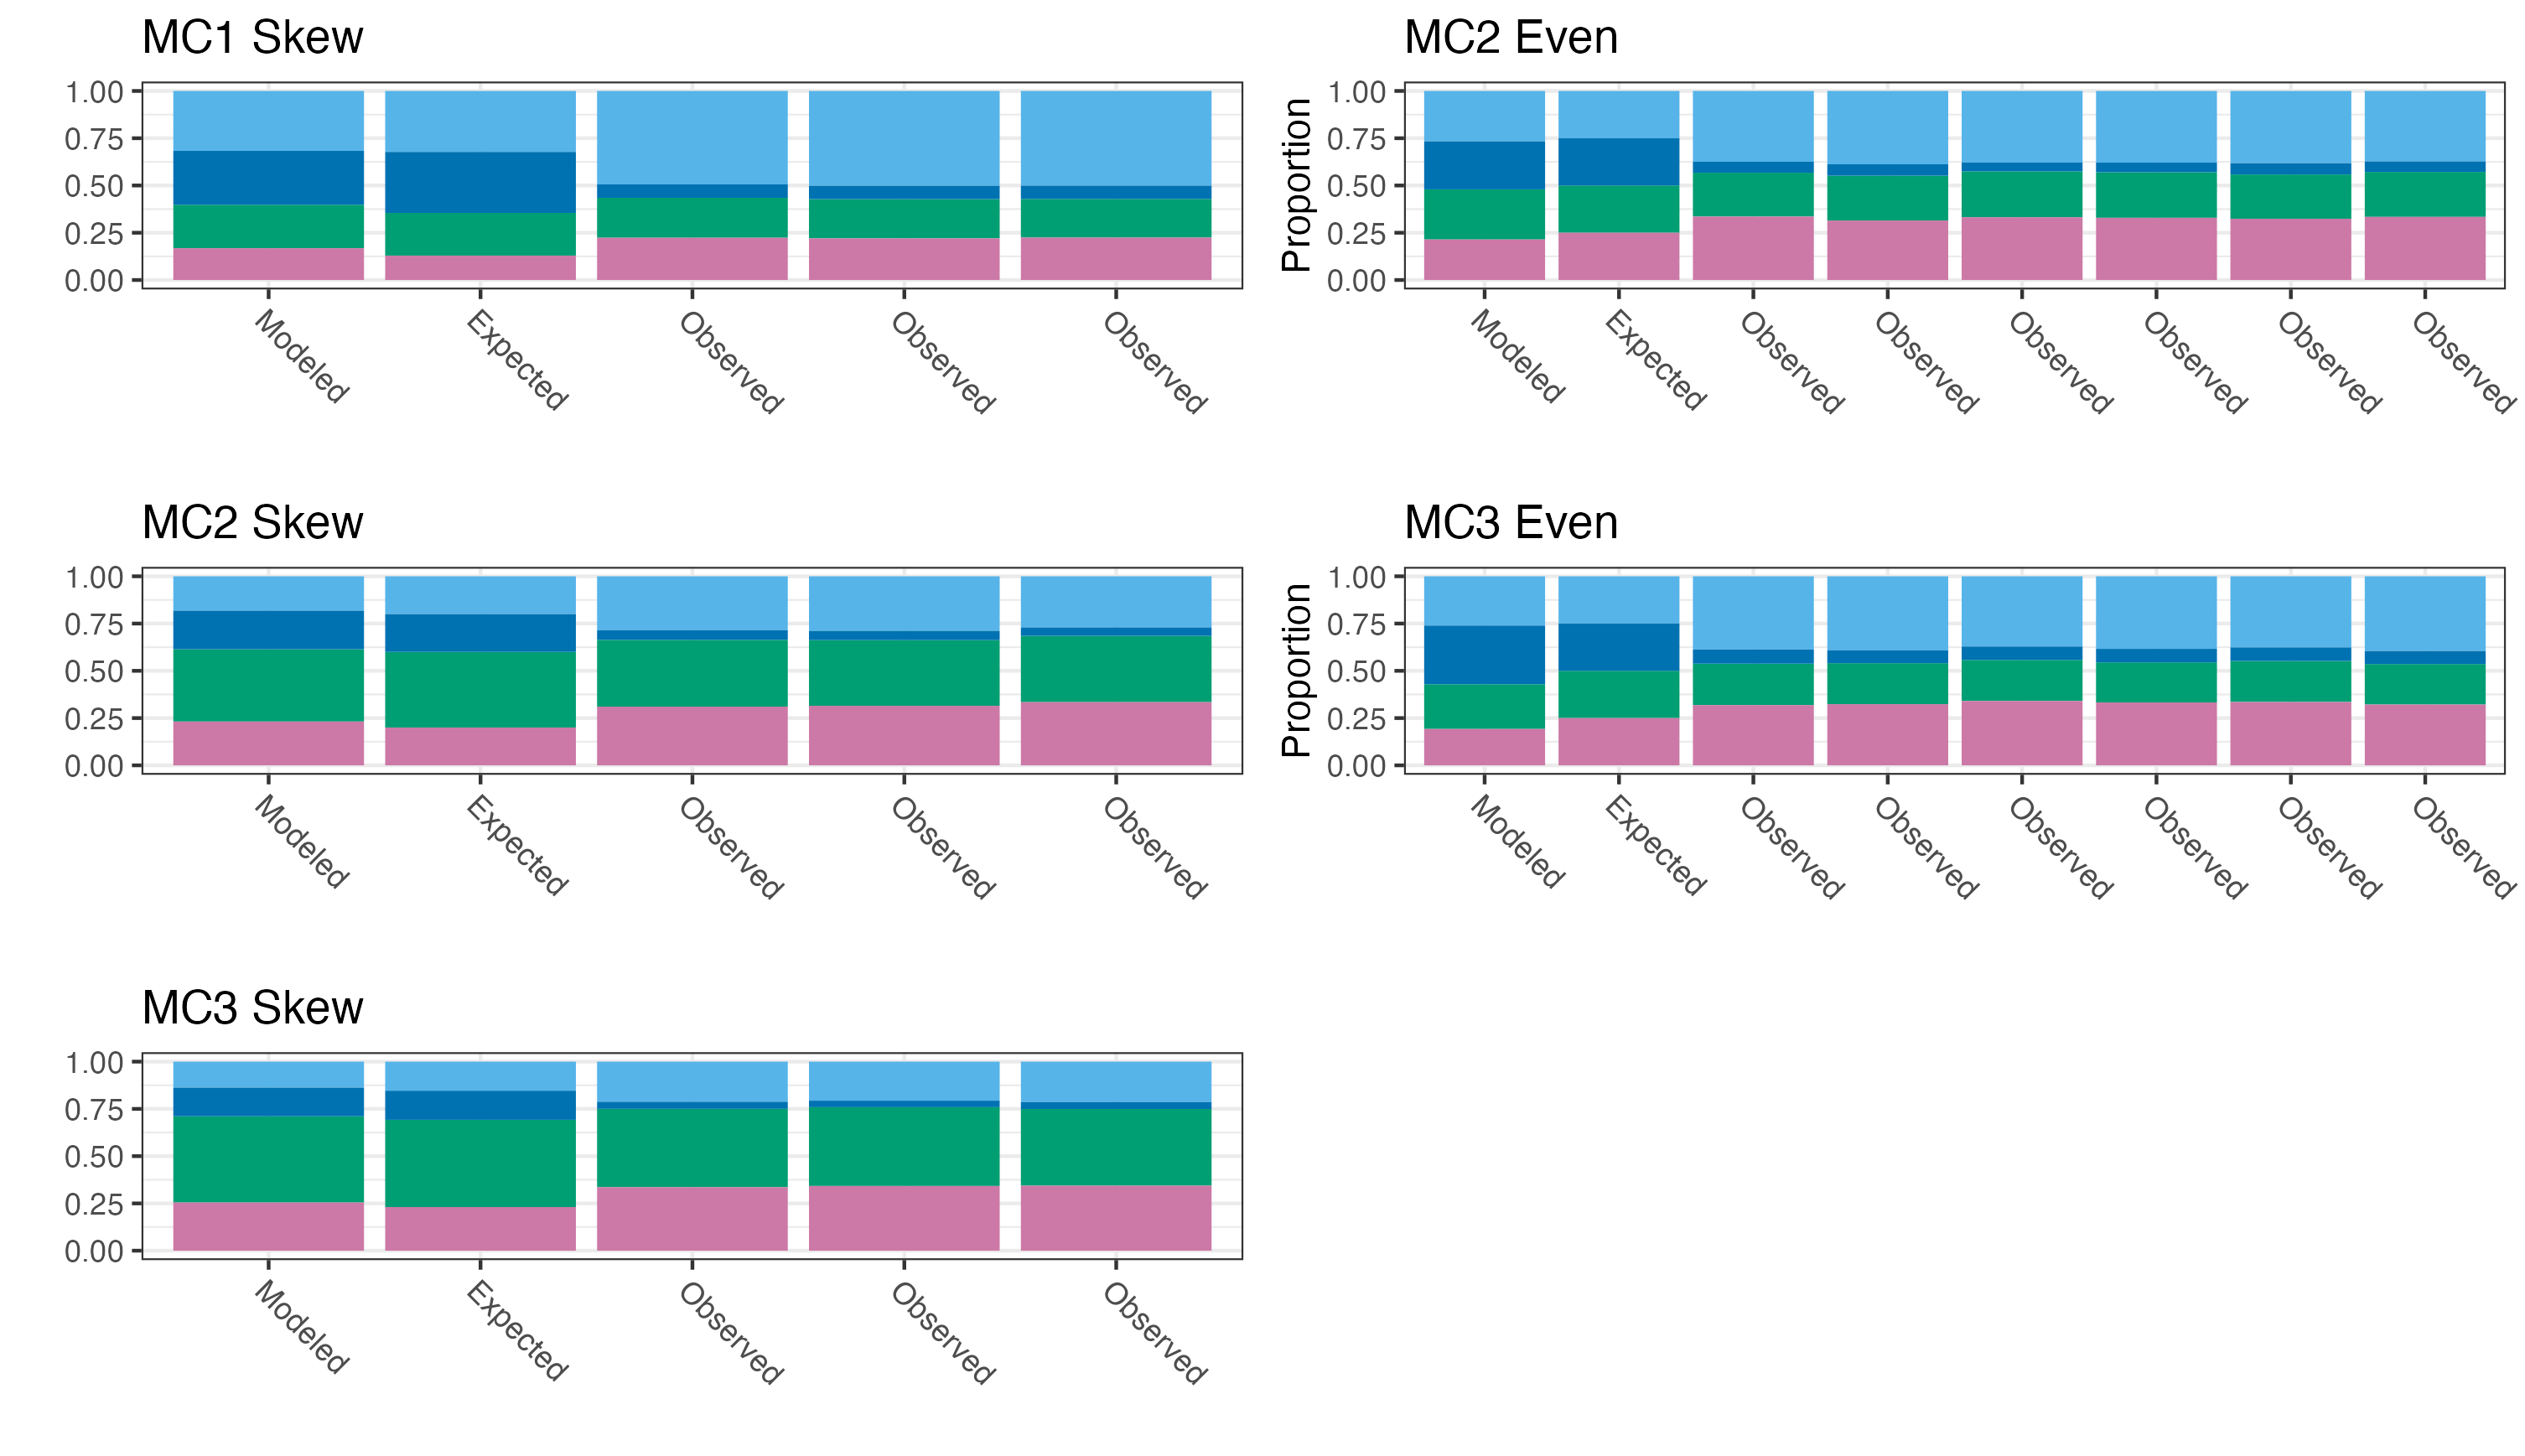
\includegraphics{../Output/SupplementalFigures/mock_internal_calibration.png}
\caption{Figure S1.10. Intercalibration of mock communities used to
correct environmental samples for amplification
bias.\label{fig:intercal}}
\end{figure}

We can also check how well the calibration is working by comparing the
alpha values by using different subsets of mock community data as true
and unknown (Figure S1.\ref{fig:alphas}). We can then use the mock
communities to correct the data from the MiSeq to account for the
different alpha values. The corrected results are shown in the main text
as Figure 4.

\begin{figure}
\centering
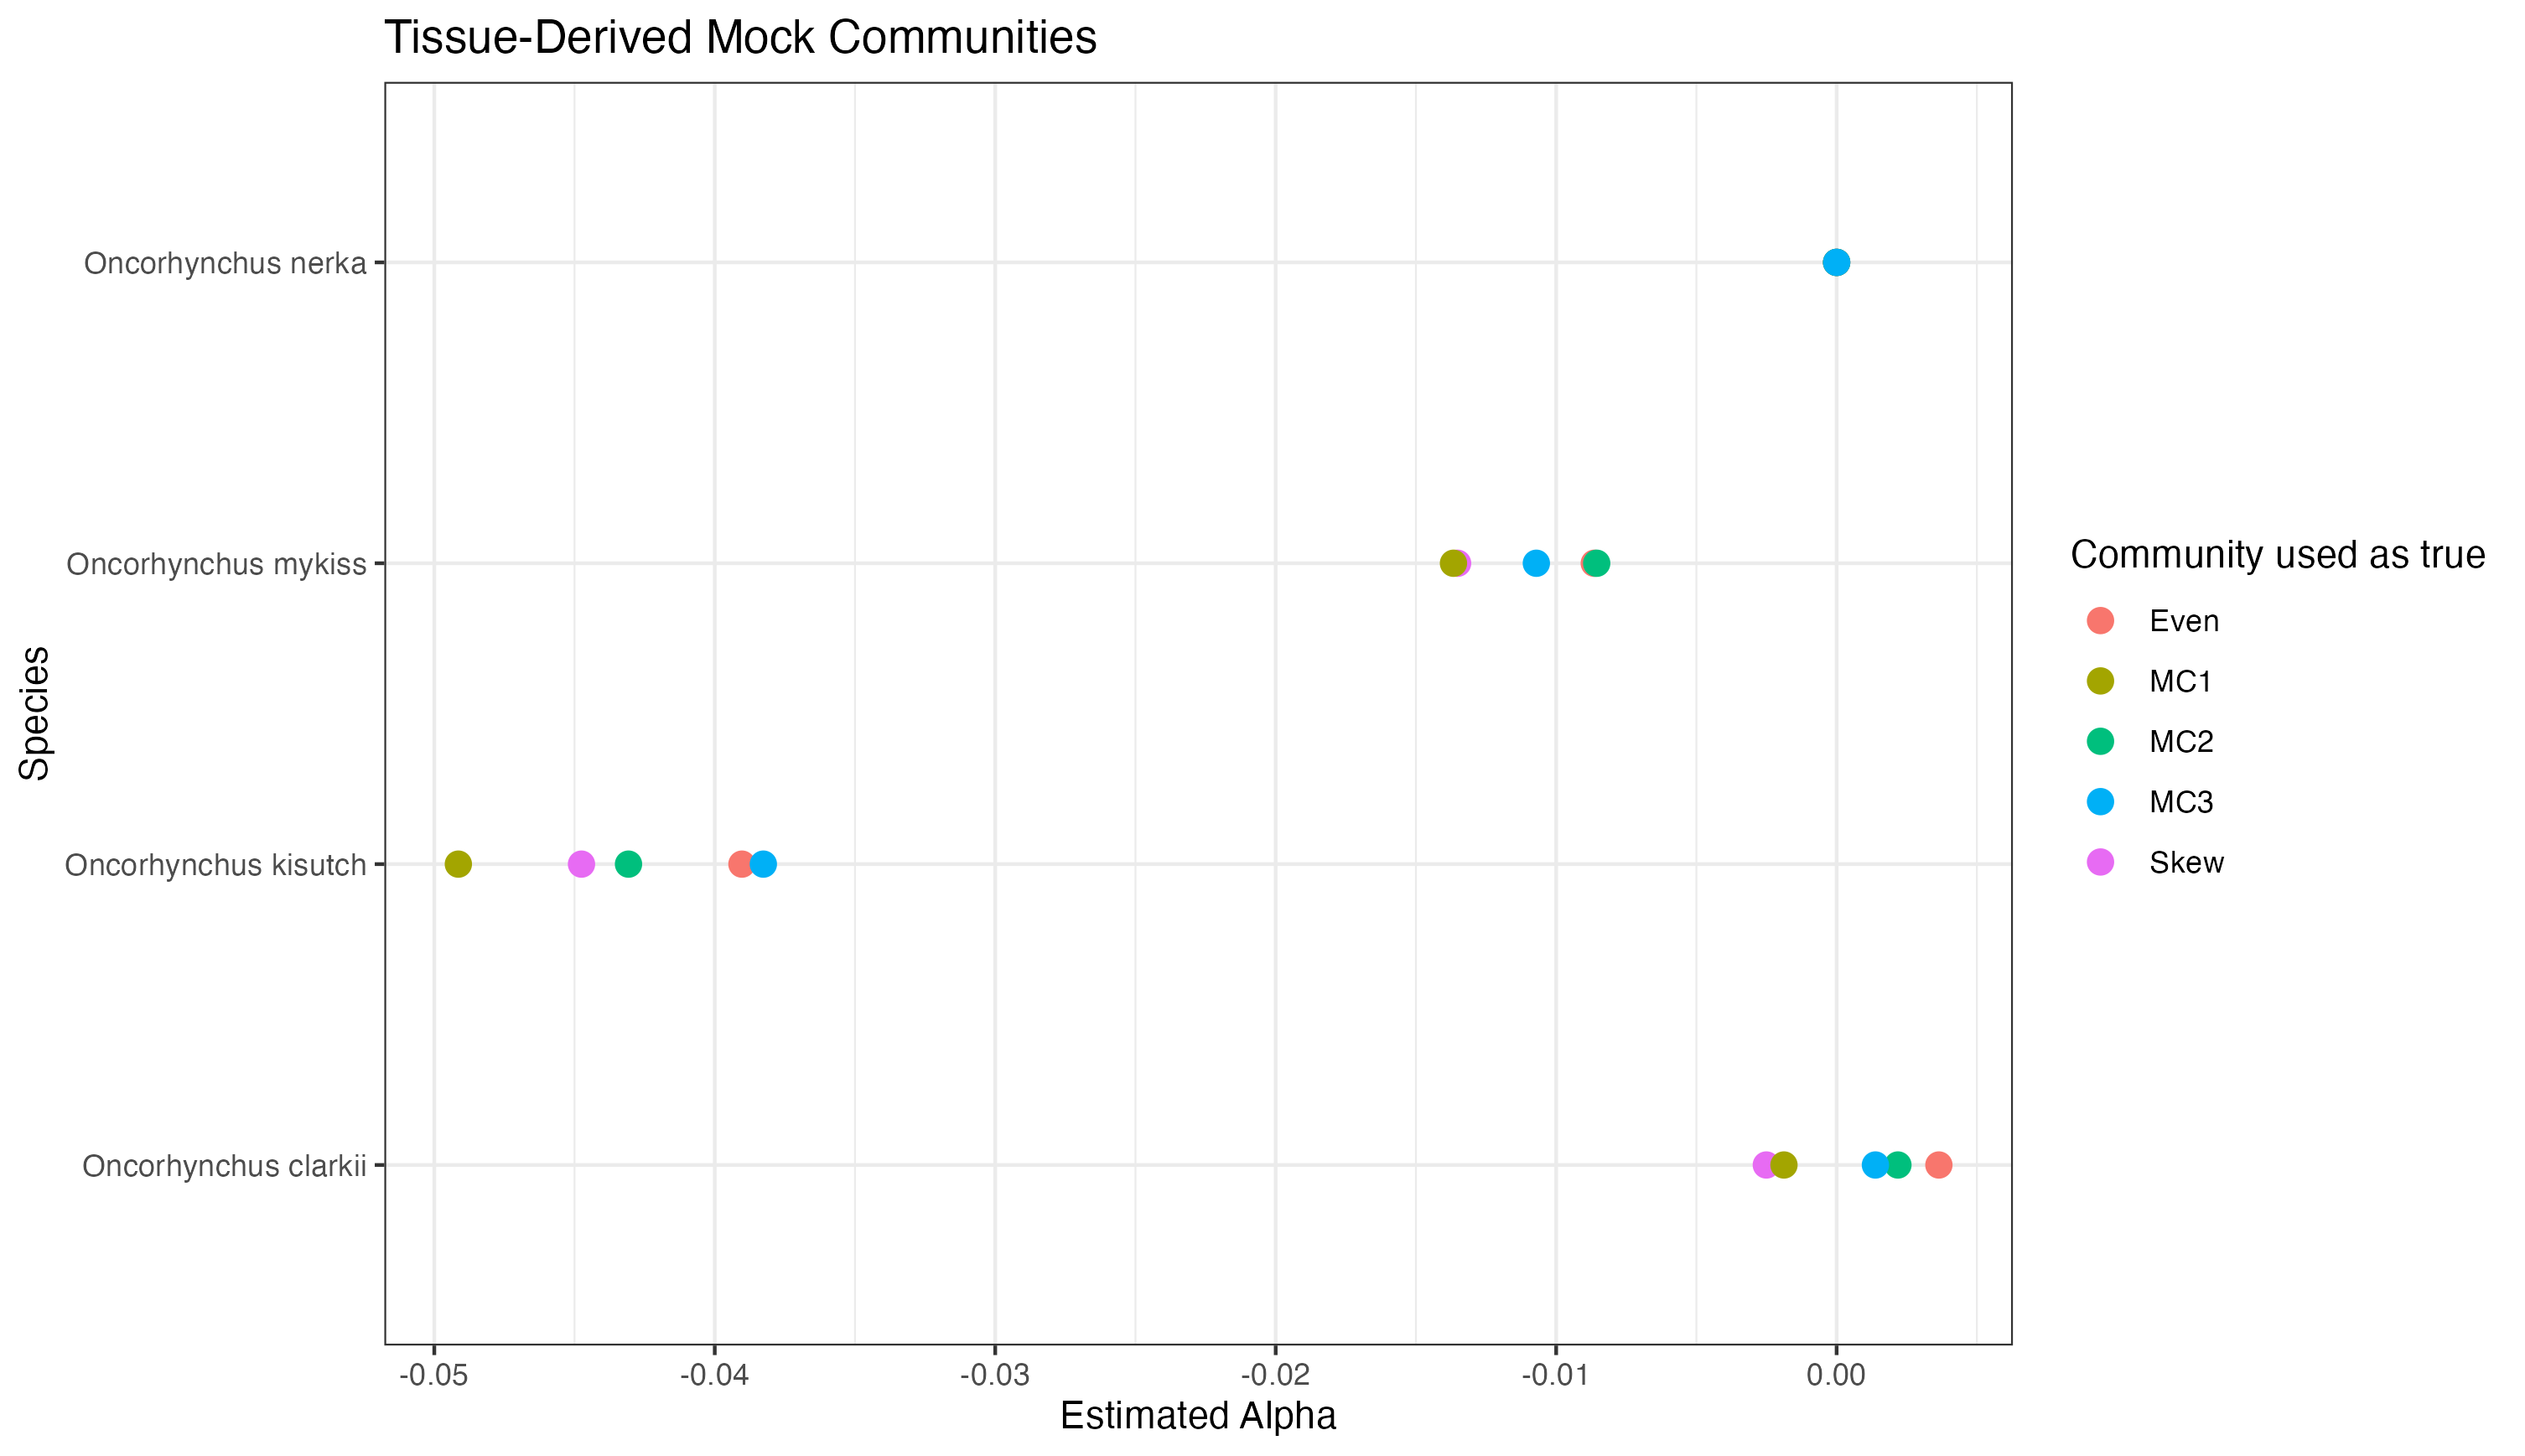
\includegraphics{../Output/SupplementalFigures/mock_internal_calibration_compare_alphas.png}
\caption{Figure S1.11. Estimated alpha values of salmonid species with
different calibrations of the mock communities. Each color represents a
different subset of mock community data treated as `true' to calibrate
the remainder of the mock community data.\label{fig:alphas}}
\end{figure}

\hypertarget{species-specific-effect-of-culverts}{%
\subsection{Species-specific Effect of
Culverts}\label{species-specific-effect-of-culverts}}

In the main text, we show the effect of culverts averaged over creeks
and species (Figure 8). Here, we show them separated by species and
creek (Figure S1.\ref{fig:culvertsspeciescreek}).

\begin{figure}
\centering
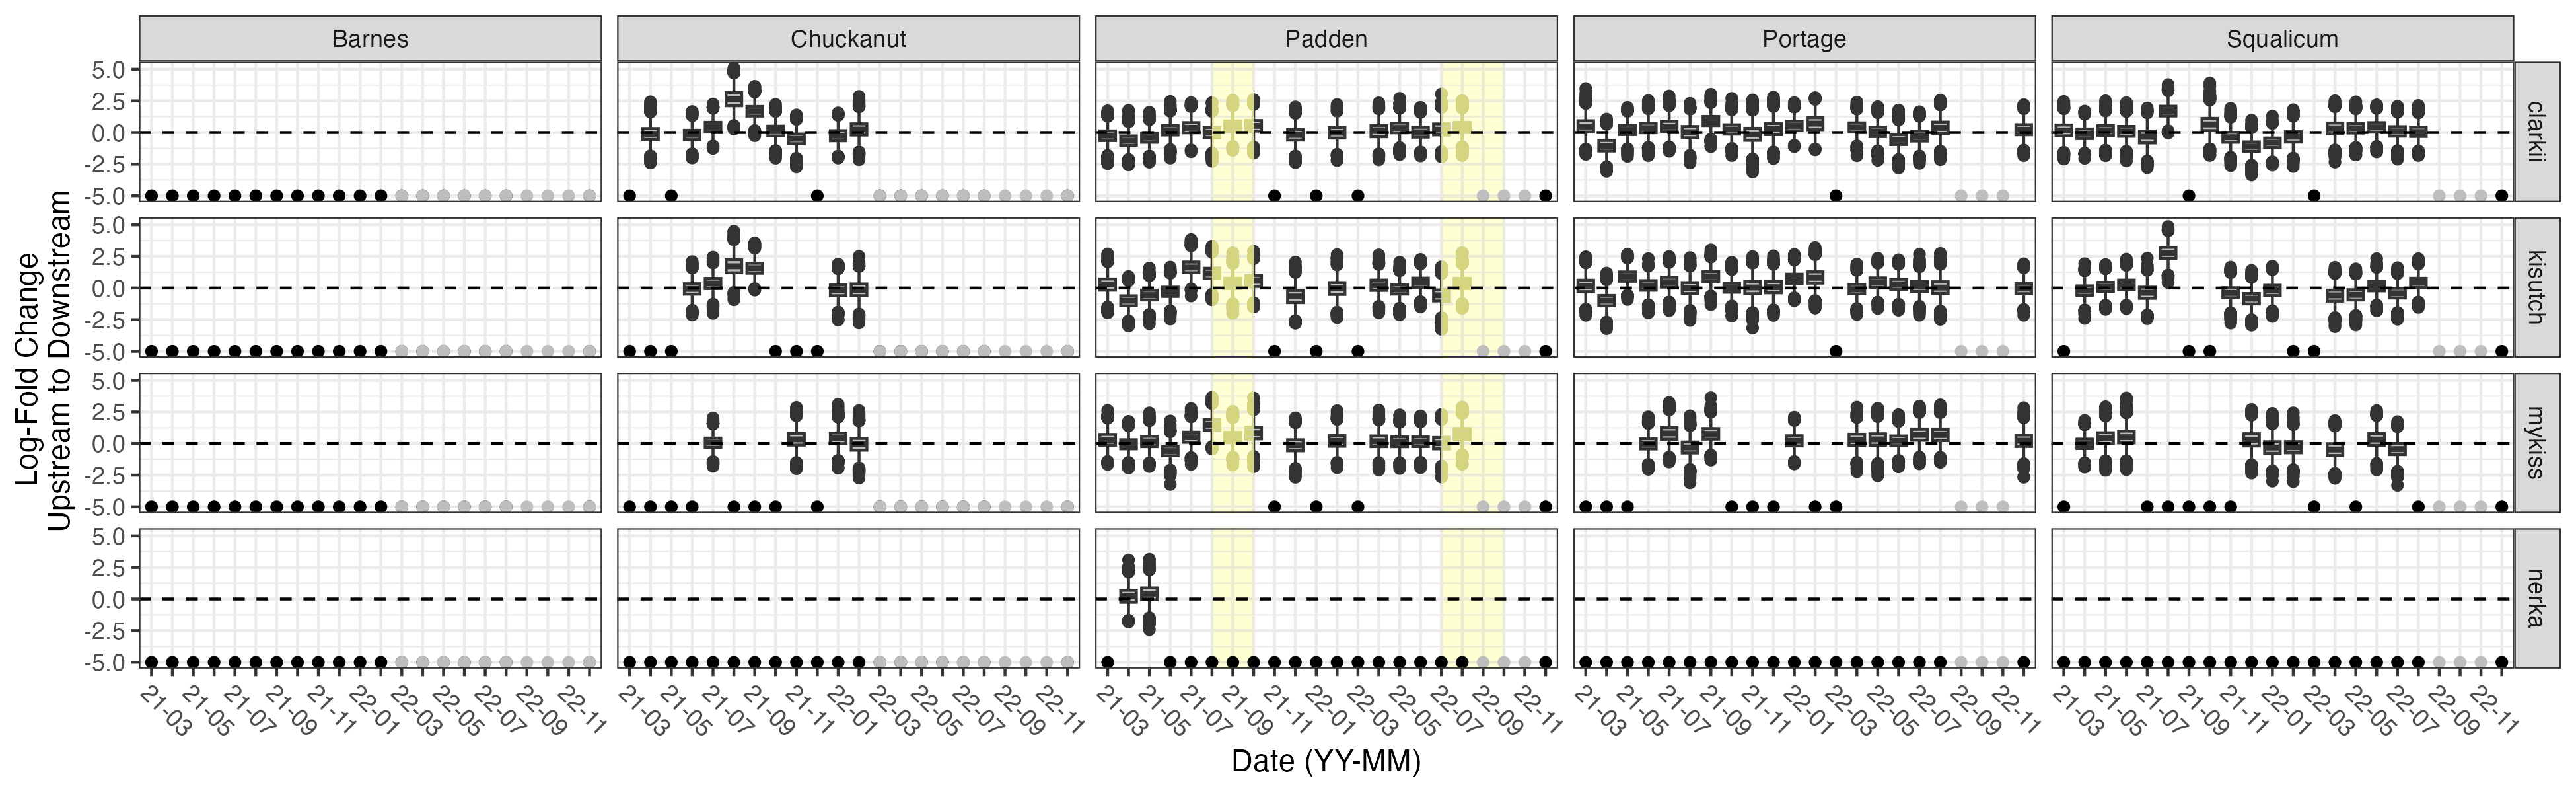
\includegraphics{../Output/SupplementalFigures/culvert_boxplot_separated.png}
\caption{Figure S1.12. The effect of culvert on salmonid abundance
separated by species and creeks across time. The y-axis shows the
log-fold change in eDNA mass flow rate (copies/s) between upstream and
downstream, normalized by upstream mass flow rate. The box boundaries
correspond to the 25th and 75th percentiles; the whiskers correspond to
1.5 times the interquartile range. Here, negative values imply that eDNA
mass flow rates are higher downstream than upstream. Samples with very
low eDNA mass flow rates (\textless{} 150 copies/s) were removed before
plotting to remove extreme proportional values due to large
denominators. Grey points indicate times when no samples were taken.
Black points indicate times when samples were taken, but no target DNA
was found in either upstream or downstream samples and therefore the
log-fold change can not be calculated.\label{fig:culvertsspeciescreek}}
\end{figure}

\hypertarget{references}{%
\subsection*{References}\label{references}}
\addcontentsline{toc}{subsection}{References}

\hypertarget{refs}{}
\begin{CSLReferences}{1}{0}
\leavevmode\vadjust pre{\hypertarget{ref-callahan2016a}{}}%
Callahan, B. J., P. J. McMurdie, M. J. Rosen, A. W. Han, A. J. A.
Johnson, and S. P. Holmes. 2016.
\href{https://doi.org/10.1038/nmeth.3869}{DADA2: High resolution sample
inference from illumina amplicon data}. Nature methods 13:581--583.

\leavevmode\vadjust pre{\hypertarget{ref-duda2021}{}}%
Duda, J. J., M. S. Hoy, D. M. Chase, G. R. Pess, S. J. Brenkman, M. M.
McHenry, and C. O. Ostberg. 2021.
\href{https://doi.org/10.1002/edn3.134}{Environmental DNA is an
effective tool to track recolonizing migratory fish following
large-scale dam removal}. Environmental DNA 3:121--141.

\leavevmode\vadjust pre{\hypertarget{ref-martin2011a}{}}%
Martin, M. 2011. \href{https://doi.org/10.14806/ej.17.1.200}{Cutadapt
removes adapter sequences from high-throughput sequencing reads}.
EMBnet.journal 17:10.

\leavevmode\vadjust pre{\hypertarget{ref-shelton}{}}%
Shelton, A. O., Z. J. Gold, A. J. Jensen, E. D'Agnese, E. Andruszkiewicz
Allan, A. Van Cise, R. Gallego, A. Ramón-Laca, M. Garber-Yonts, K.
Parsons, and R. P. Kelly. 2022.
\href{https://doi.org/10.1002/ecy.3906}{Toward quantitative
metabarcoding}. Ecology n/a:e3906.

\leavevmode\vadjust pre{\hypertarget{ref-thomas2018a}{}}%
Thomas, A. C., J. Howard, P. L. Nguyen, T. A. Seimon, and C. S.
Goldberg. 2018. ANDe {\texttrademark}: A fully integrated environmental
DNA sampling system. Methods in Ecology and Evolution 9:13791385.

\leavevmode\vadjust pre{\hypertarget{ref-thomas2019}{}}%
Thomas, A. C., P. L. Nguyen, J. Howard, and C. S. Goldberg. 2019.
\href{https://doi.org/10.1111/2041-210X.13212}{A self-preserving,
partially biodegradable eDNA filter}. Methods in Ecology and Evolution
10:1136--1141.

\leavevmode\vadjust pre{\hypertarget{ref-washingtondepartmentoffishandwildlife2019}{}}%
Washington Department of Fish and Wildlife. 2019. Fish passage
inventory, assessment, and prioritization manual.

\leavevmode\vadjust pre{\hypertarget{ref-wilkinson2018}{}}%
Wilkinson, S. P., S. K. Davy, M. Bunce, and M. Stat. 2018.
\href{https://doi.org/10.7287/peerj.preprints.26812v1}{Taxonomic
identification of environmental DNA with informatic sequence
classification trees.}

\end{CSLReferences}

\end{document}
